\documentclass[twocolumn,superscriptaddress,aps,nofootinbib]{revtex4-1}

\usepackage[utf8]{inputenc}

\usepackage{amsfonts}
\usepackage{amssymb}
\usepackage{amsmath}
\usepackage{amsthm}

\usepackage{enumitem}
\usepackage{csquotes}

\usepackage{bbold}
\usepackage{bm}
\usepackage{graphicx}
\usepackage{color}
\usepackage{hyperref}

\usepackage{multirow}
\renewcommand{\arraystretch}{1.2}

\usepackage[binary-units = true]{siunitx}
\DeclareSIUnit\px{px}

\begin{document}


% ==============================================================================

\title{\Large{Automatic Detection Of Photovoltaic Panels Through Remote Sensing}}
\vspace{1cm}
\author{\small{\bf Yann Claes}}
\affiliation{\texttt{yann.claes@student.uliege.be} (\texttt{s161317})}
\author{\small{\bf Gaspard Lambrechts}}
\affiliation{\texttt{gaspard.lambrechts@student.uliege.be} (\texttt{s161826})}
\author{\small{\bf François Rozet}}
\affiliation{\texttt{francois.rozet@student.uliege.be} (\texttt{s161024})}
\maketitle

% ==============================================================================

\section{Introduction}
Nowadays, photovoltaic (PV) panels play an important role in the transition towards renewable energy production, and more and more small/large-scale PV systems are installed worldwide. Their major strength is that anyone owning a rooftop/open field can install PV panels, hence can produce electricity in a renewable fashion.

Nevertheless, this growth also makes it very hard to estimate their geographical deployment, and it is thus hard to assess the production capacity of a given region, which influences exchanges in electrical grids.

By having access to some estimate of the production capacity of any region, one could easen the decisions made about the amounts of energy that should be produced from any possible source (nuclear, coal, etc.), to satisfy the total demand.

Therefore, this project, which we named ADOPPTRS for \emph{Automatic Detection Of Photovoltaic Panels Through Remote Sensing}, aims at assessing the PV production capacity of a specific region using deep neural networks and aerial/satellite images processing. With these, our goal is to provide reliable estimates of all existing panels installations' locations and areas. More specifically, we want to apply our model(s) to the images of the \href{https://geoportail.wallonie.be/walonmap}{WalOnMap} website\footnote{This project was conducted in parallel with our \emph{Big Data} project.}.

Section \ref{sec:related_work} will cover research related to our problem. Section \ref{sec:methods} explains in details the different neural network architectures we reproduced/extended, along with the loss functions and optimizers we used. It will also present the data (pre-)processing and augmentation performed.
Section \ref{sec:results} introduces our experimental procedure and the experiments we conducted along with their results.
Finally, section \ref{sec:discussion} concludes with a critical analysis of the results and some further developments or improvements we did not explore.

\section{Related work}\label{sec:related_work}

The DeepSolar \cite{yu2018deepsolar} project represents our main source of inspiration. Indeed, this project shares the same goals as ours : predicting the locations and areas of solar panels, using deep learning frameworks. With their project, the authors of DeepSolar constructed a comprehensive and publicly available database of solar installations in the United States. Out of the scope of our project, they were able to highlight interesting correlations between photovoltaic development and environmental as well as socioeconomic factors, such as income and inequalities.

Their model uses 2 branches. The first one is a CNN classifier (Google Inception V3 \cite{szegedy2016rethinking}) used to detect the presence or absence of PV panels in the processed image. The second one is also a CNN that is connected to the intermediate layers of the first branch to perform segmentation and estimate the size and shape of the detected panels.

Other PV panels detection and segmentation tasks were already developed in the past. For instance, in \cite{yuan2016large}, they used a very simple CNN architecture to solve their problem. It consists of a combination of convolutional layers, max-pooling layers and up-sampling layers. They also used a signed distance function of boundaries, which helps the network to better identify solar panels.

In \cite{malof2016automatic} and \cite{malof2016deep}, they detect PV panels in very high resolution aerial imagery, using respectively Random Forests and CNNs. Furthermore, and even more interesting for our project, they made their data set publicly available \cite{bradbury2016distributed}, providing more than \num{19000} human-annotated locations over \num{601} images of four cities in California, covering a total spatial area of \SI{1350}{\kilo\meter\squared}.

In a more general and broader point of view, U-Net \cite{ronneberger2015u} and SegNet \cite{badrinarayanan2017segnet} can be considered as pillars in image segmentation tasks. Both rely on convolutional layers along with max-pooling and up-sampling layers, even though there are still important differences between both architectures. Since they are both networks we reproduced (to some extent), we will detail them in section \ref{sec:methods}.

\section{Methods} \label{sec:methods}

\subsection{Architectures}

All model implementations can be found in the source code \texttt{python/models.py}.

All implemented neural networks are (fully) convolutional neural networks. They are used as \emph{segmentation} networks, meaning that their goal is to transform the image tensor (3 channels) into other tensors successively, until creating a final mask tensor of $C$ channels that tells for each pixel the probability it belongs to each class in $C$. In our case, we only have 2 classes : being a PV pixel, or being another pixel. Thus, we decided to only have 1 channel instead of 2 in the final tensor : the probability of being a PV pixel $p$ ; the other class having probability $1 - p$. These convolutional neural networks will use the following types of layers, \emph{i.e.} transformations from one tensor to another :
\begin{description}[leftmargin=*]
    \item[Convolutional] A convolutional layer transforms a $C$-channels tensor into a $D$-channels one. Each new channel is associated with a different \emph{kernel} of shape $C \times w \times h$. Each element $(i, j)$ in a (new) channel is computed as the the sum of the elements of the element-wise product of its kernel and a $C \times w \times h$ window \enquote{surrounding} $(\cdot, i, j)$ in the previous tensor. This process is called a \emph{convolution}.

    In addition, it is possible to add a \emph{padding}, \emph{i.e.} additional bordering elements, to the original image to avoid (or decrease) the reduction of size in the output tensor. Indeed, without padding, if $w$ and/or $h$ are greater than $1$, it is not possible to apply the convolution to the border elements, and therefore the output tensor shrinks.

    A \emph{stride} can also be used in order to reduce explicitly the dimension of the tensor (down-sampling) by translating the kernel several elements at a time (horizontally and vertically) instead of one by one.

    In our implementations, we will use $C \times 3 \times 3$ and $C \times 1 \times 1$ kernels with a respective padding of $1$ and $0$, but no stride, such that only the number of channels varies.
    \item[Pooling] A pooling layer reduces the tensor dimensions but not the number of channels. This is done by considering a kernel of shape $w \times h$ that has a stride of $(w, h)$, so that no overlapping exists between the considered windows. Then, on each of these windows is applied a non linear function, called a \emph{filter}, instead of a weighted sum like in the convolutional layer.

    In our case, we will only consider the simple \emph{max pooling layer}. It means that for each window we simply keep the maximum value. This is done independently in each channel, unlike in convolutional layers.
    \item[Up-sampling] An up-sampling layer increases the tensor dimensions (but not the channels). In our implementations, we use two types of up-sampling layers :
    \begin{enumerate}[leftmargin=*]
        \item \emph{Classic up-sampling layers}, where the dimensions of the tensor are increased by a factor $(w, h)$. To fill in all new elements, an interpolation technique must be used. In our implementations, we use the \emph{bilinear} up-sampling. Starting from the four surrounding known elements, it first performs a linear interpolation in one direction, obtaining rows (or columns) of filled elements, and then another one in the other direction; the resulting interpolation is thus nonlinear, in fact quadratic.
        \item \emph{Pooling indices up-sampling layers} are used in parallel with a \emph{max pooling} layer. They revert the max pooling operation by creating a tensor of the original shape filled with zeros except at the \emph{positions} corresponding to elements that were selected as maximum by the \emph{max pooling}. At these positions, the values of the input tensor are used. \emph{N.B.} This input tensor does not necessarily contain the values of the max-pooling.
    \end{enumerate}
    \item[ReLU] A layer that puts all negative elements to zero, which introduces (beneficial) nonlinearities.
    \item[Sigmoid] A layer that applies the sigmoid function
    \begin{equation}
        \sigma(x) = \frac{1}{1 + \exp(-x)}
    \end{equation}
    to every element.
    \item[Softmax] A layer that applies the channel-wise sigmoid function to every element, \emph{i.e.}
    \begin{equation}
        t_{kij} \leftarrow \frac{\exp(t_{kij})}{\sum_{l=1}^C \exp(t_{lij})}
    \end{equation}
    with $\bm{t}$ a tensor in $\mathbb{R}^{C \times W \times H}$ and $k$, $i$, $j$ indices respectively $\leq C$, $\leq W$ and $\leq H$.

    The interesting property of this transformation is that, afterwards,
    \begin{equation}
        \sum_{k=1}^C t_{kij} = 1
    \end{equation}
    similarly to probabilities.
    \item[Batch normalization] A batch normalization layer improves performance and stability of the network, often allowing to achieve similar or better performance with much less training epochs. Most of the time, and according to the original paper \cite{ioffe2015batch}, it consists in an additional layer between a convolutional layer and an activation layer (like ReLU). Its role is to shift and rescale the current (mini-)batch according to the moments (mean and variance) estimated during the \emph{training} phase. If its benefits have been demonstrated many times, there is yet no consensus on the reasons of its effectiveness.

    \emph{N.B.} In an early stage of our implementations, we used both Batch Normalization (BN) and Dropout \cite{srivastava2014dropout}, but it seemed to cause some convergence problems. We decided to remove the latter, as it slows down training. Furthermore, some papers, including \cite{ioffe2015batch}, suggest that Batch Normalization could, in some cases, eliminate the need for Dropout or even interfere with it \cite{li2019understanding}. It should be noted that we haven't performed a rigorous analysis of this behaviour, as it was not the subject of our project.
\end{description}

With these layers, four architectures have been implemented.

\vspace{1em}

\paragraph{U-Net}

The first model we implement (based on \cite{usuyama2018unet}) is U-Net \cite{ronneberger2015u}, which is known for biomedical image segmentation. Its architecture consists in a downhill path followed by an uphill path, depicted on FIG. \ref{fig:unet_architecture}.

\begin{figure}[h]
    \centering
    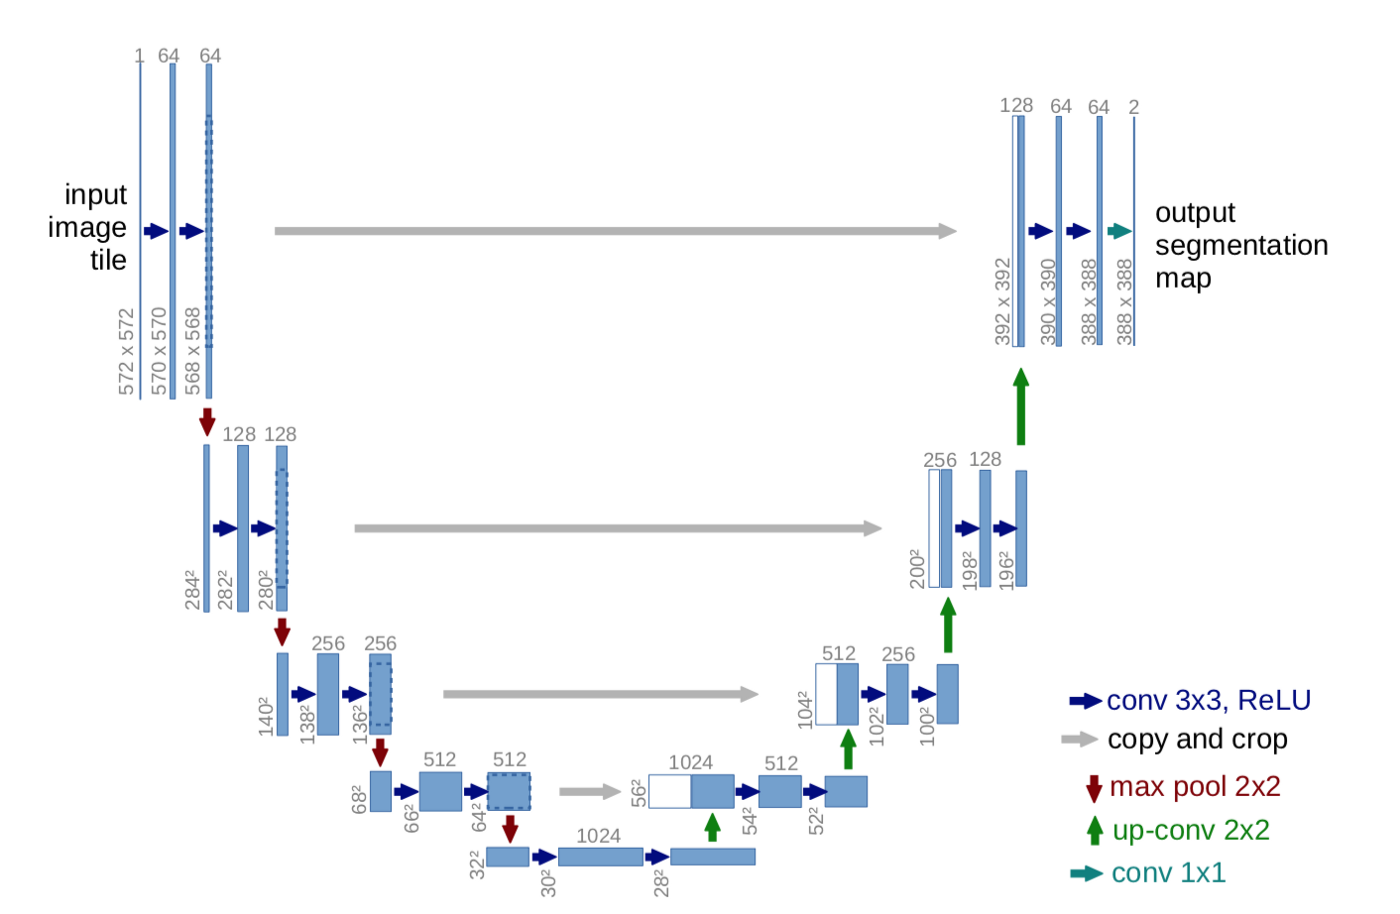
\includegraphics[width=\columnwidth]{resources/png/unet_architecture.png}
    \caption{Original U-Net architecture. \cite{ronneberger2015u}}
    \label{fig:unet_architecture}
\end{figure}

The downhill path of the original U-Net is made of 5 successive \emph{double convolutions} interleaved with $2 \times 2$ max-pooling. Each convolution is composed, in that order, of
\begin{itemize}[noitemsep]
    \item A 2-D padded\footnote{It should be noted that, in the original implementation, there was no padding.} convolution with a kernel of size $C \times 3 \times 3$;
    \item A ReLU activation function.
\end{itemize}
We keep the same structure for the double convolution operation but have added a batch normalization layer between the convolution and the ReLU in order to improve convergence and stability; this will be discussed in section \ref{sec:results}.

Similarly to the original architecture (FIG. \ref{fig:unet_architecture}), we double the number of channels at each double convolution, except the first time where we move from 3 channels to 64. At the same time, the dimensions of the image are divided by two due to the max-pooling after each double convolution. Note that the fifth double convolution operation is not followed by a max-pooling afterwards.

At the end, the feature map is thus composed of $64 \times 2^4 = 1024$ channels with dimensions that depend on the input image dimensions, but that are $2^4 = 16$ times smaller.

The uphill path consists of 4 repetitions of the following layers :
\begin{itemize}
    \item An up-sampling of the feature maps, with a scale factor of 2. This means that the resulting output feature map will be twice as big (along each dimension) as the down-sampled feature map. As up-sampling method, we use the bilinear up-sampling;
    \item A concatenation with the corresponding feature map along the channel axis;
    \item A \emph{double convolution} (with batch normalization) such that the number of channels is divided by three.
\end{itemize}
Hence, at each up-sampling step, the number of channels is divided by two because the concatenation increase the number of channels by \num{1.5}, while the dimensions are doubled.
In our case, since we use a padding of \num{1}, consistently with the kernel of shape $C \times 3 \times 3$, we do not need to crop the feature maps before concatenating them with the up-sampled feature map.

The concatenation with the corresponding feature map is in fact a \emph{passthrough} connection that allows the successive up-sampled feature maps to benefit from the more \emph{local} features present in the feature maps of the downhill path (see gray arrows in FIG. \ref{fig:unet_architecture}).

Finally, there is the last layer. The original network uses a $1 \times 1$ convolution to map each feature vector to the appropriate number of classes. In our network, we use the same layer followed by a sigmoid activation to obtain a prediction of the likelihood that a pixel is within a PV panel.

\vspace{1em}

\paragraph{SegNet}

The second model we reproduce is SegNet \cite{badrinarayanan2017segnet}. As described in the paper, SegNet is composed of an encoder network, a decoder network and a pixelwise classification layer.

In the original architecture, as can be seen on FIG. \ref{fig:segnet_original_architecture}, the encoder consists of 13 convolutional layers, arranged precisely in the following way:
\begin{itemize}
    \item[$2\, \times$] a \emph{double convolution}, the same as in U-Net (with batch normalization), followed by a max-pooling layer retaining the pooling indices for later up-sampling.
    \item[$3\, \times$] a \emph{triple convolution}, which is identical to double convolution except that it has 3 convolutions instead of 2.
\end{itemize}

\begin{figure}[h]
    \centering
    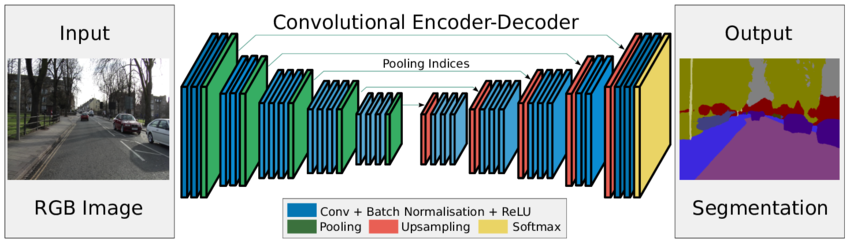
\includegraphics[width=\columnwidth]{resources/png/segnet_architecture.png}
    \caption{Original SegNet architecture. \cite{badrinarayanan2017segnet}}
    \label{fig:segnet_original_architecture}
\end{figure}

The decoder is the symmetrical counterpart of the encoder, using pooling indices up-sampling layers instead of pooling layers. It differs from U-Net as it doesn't rely on \emph{concatenation} but rather on pooling indices to carry information.

However, for this project, we do not to use the full SegNet architecture. Rather, we reproduce a smaller SegNet \cite{camilo2018application}, dropping all triple convolutions and using 3 layers of double convolution, each followed by a max-pooling layer, for the downhill path. This architecture is depicted on FIG. \ref{fig:segnet_truncated}.

\begin{figure}[h]
    \centering
    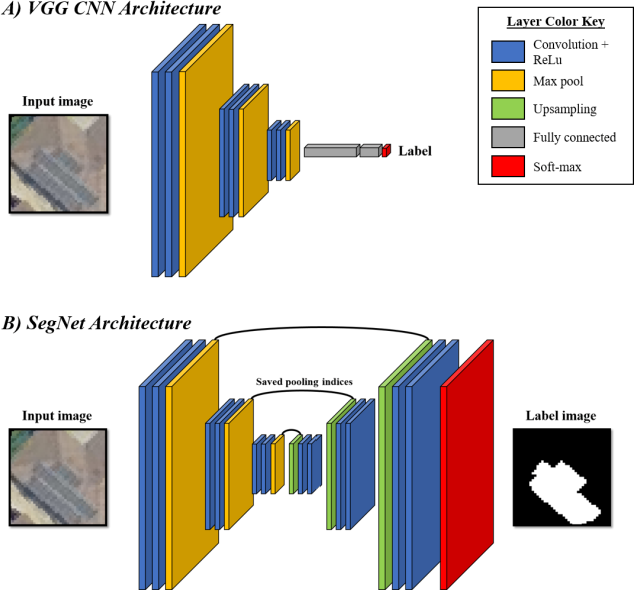
\includegraphics[width=\columnwidth]{resources/png/segnet_truncated.png}
    \caption{Truncated version of SegNet. \cite{camilo2018application}}
    \label{fig:segnet_truncated}
\end{figure}

As far as the number of convolutional filters in the convolutional layers are concerned, it is similar to \cite{camilo2018application}, \emph{i.e.}
\begin{itemize}[noitemsep]
    \item The first \emph{double convolution} moves from 3 channels to 64 channels;
    \item The second one increases the number of channels to 128;
    \item The third one keeps the number of channels equal to 128.
\end{itemize}
As explained above for the general SegNet architecture, the decoder is simply the symmetrical counterpart of these 3 layers, and makes use of pooling indices for its up-sampling layers. Hence, its first \emph{double convolution} layer keeps the number of channels at 128, its second one moves to 64 channels while the last one moves to a single channel.

In addition, as final layer, we use a $1 \times 1$ convolutional layer followed by a sigmoid activation, highlighting the presence/absence of panel.

One can notice the similarities between U-Net and Segnet. Indeed, except for the number of hidden layers, they present the same idea of a down-sampling downhill path followed by an up-sampling uphill path that uses \emph{passthrough} connections to gather prior information.

The difference lies in the way this information is carried. Indeed, in U-Net it is done by concatenating the feature maps, while, in SegNet, the only information comes from the max-pooling indices. The latter obviously carries less information, but is also much lighter memory-wise and complexity-wise.

\vspace{1em}

\paragraph{Multi-task U-Net}

For now, our U-Net implementation differs from the original by the following aspects
\begin{itemize}[noitemsep]
    \item Batch normalization in the double convolutions;
    \item Padding in the convolutions, removing the need for cropping the feature map in the concatenation process;
    \item Adapted to binary classification with a sigmoid layer and a single channel output;
\end{itemize}

Even if this U-Net implementation had already given us satisfying quantitative results, a qualitative analysis of the output masks has revealed that U-Net had some trouble to delimit the boundaries of the PV arrays. To overcome this issue, we got inspired by an adaptation of SegNet that specifically addresses this problem in the case of building segmentation \cite{bischke2019multi}.

In this paper, they review the classical approaches to overcome this problem, including post-processing of the mask or training MLP on top of the fully convolutional network. To avoid the difficulty of the former and the computational cost of the latter, they introduced a \emph{multi-head} fully convolutional network along with an adapted \emph{multi-task} loss and showed that this approach allowed reaching better quantitative results.

The whole idea behind this new head is to add a geometric term that incorporates the boundary information in the loss, in addition to the semantic term that is about classifying each individual pixel. This is done by trying to predict the \emph{truncated signed distance transform} of the mask, instead of the mask itself. The transformed architecture can be visualized on FIG. \ref{fig:multitask_segnet}, in the case of a Segnet encoder-decoder instead of U-Net.

\begin{figure}[h]
    \centering
    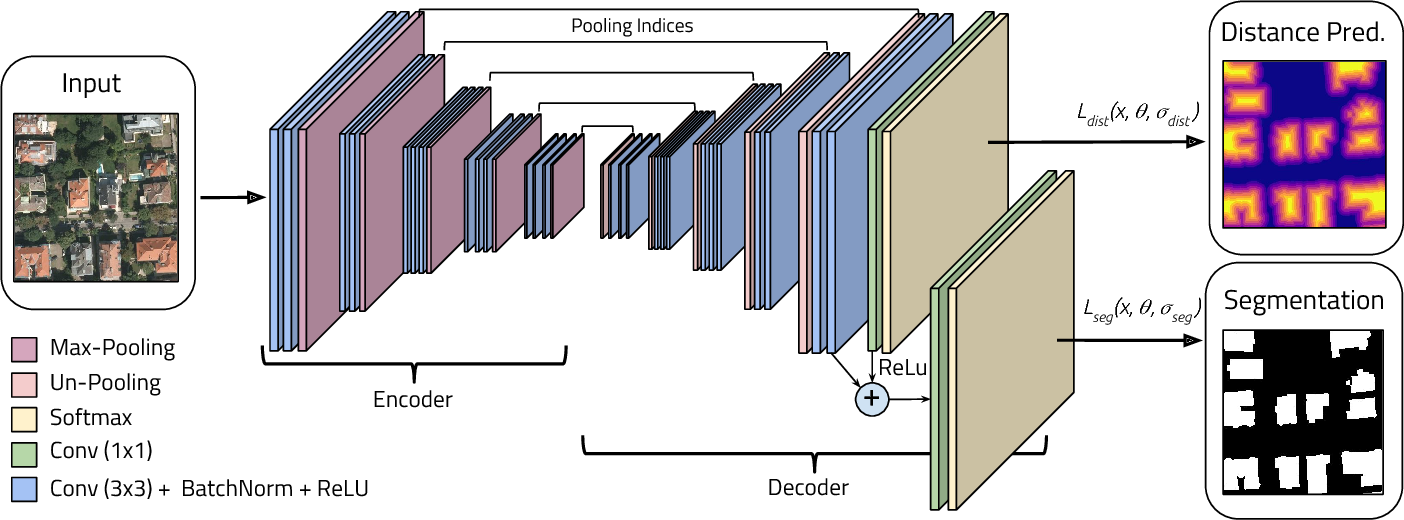
\includegraphics[width=\columnwidth]{resources/png/multitask_segnet.png}
    \vspace{-1em}
    \caption{Multi-head Segnet architecture. \cite{bischke2019multi}}
    \vspace{-0.5em}
    \label{fig:multitask_segnet}
\end{figure}

The structure of the Multi-task U-Net is exactly the same as U-Net without the last $1 \times 1$ convolutional and sigmoid layers. Instead, the distances are computed from the output of the decoder by using a $1 \times 1$ convolutional layer followed by a softmax layer. The $1 \times 1$ convolutional layer has $2R + 1$ output channels corresponding to the classes of discretized \emph{distances} (see \emph{N.B.}).

In parallel, the last layer of the decoder and the output of the aforementioned $1 \times 1$ convolutional layer -- passed through a ReLU layer -- are concatenated along the channel axis, whereupon they are passed through another $1 \times 1$ convolutional layer and sigmoid in order to produce the prediction \emph{mask}.

\emph{N.B.} The \emph{distance transform} of a mask is the map of distances of each pixel to its closest \emph{contour}. A contour is the frontier between the \num{0} and \num{1} pixels. The \emph{signed distance transform} is the distance transform, negatively signed when the pixel is a background pixel (\num{0}'s). Finally, the \emph{truncated signed distance transform} is bounded between $-R$ and $R$ and discretized into $2R + 1$ different classes. What is pleasantly surprising is that the \emph{distance transform} can be computed in \emph{linear} time.

\begin{figure}[h]
    \centering
    \vspace{-1em}
    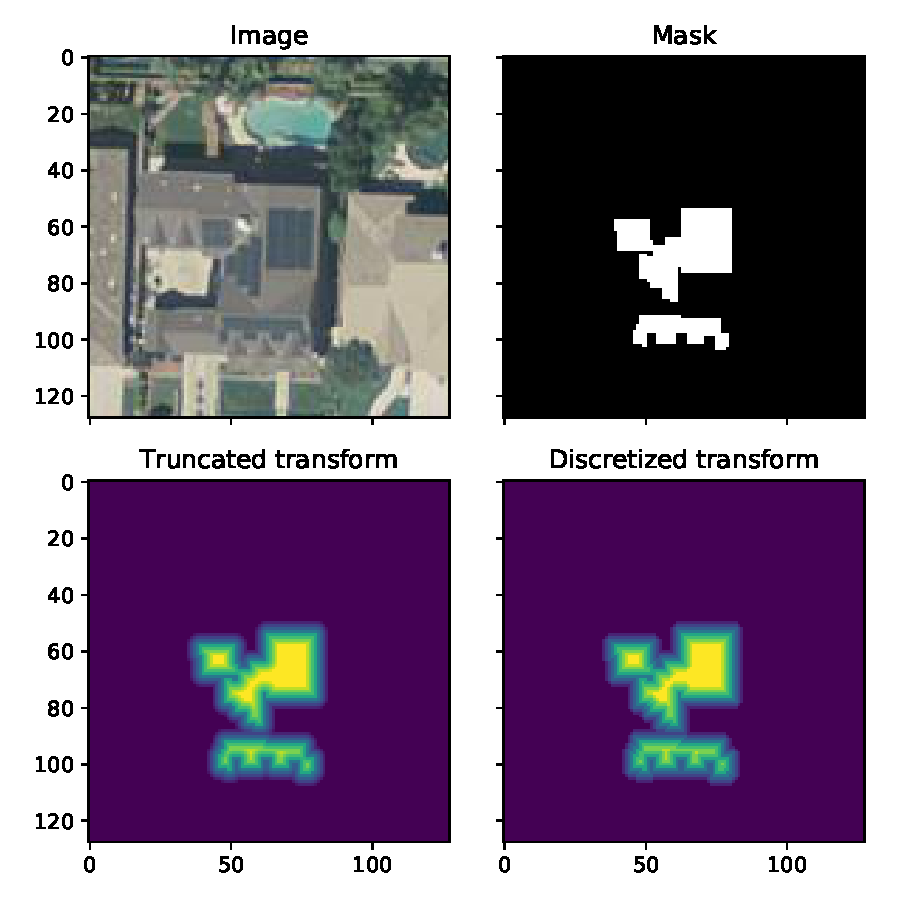
\includegraphics[width=\columnwidth]{resources/pdf/distance_transform.pdf}
    \vspace{-2em}
    \caption{Truncated distance transform representation.}
    \vspace{-0.5em}
    \label{fig:distance_transform}
\end{figure}

Formally, if $Q$ denotes the set of pixels of the contours, the truncated signed distance transform of a pixel $p$ is defined as
\begin{align}
    D(p) & = \delta_p \min \left( \min_{\forall q \,\in\, Q} d(p, q), R \right) \\
    \delta_p & = \begin{cases}
        +1 \quad & \text{if } p \in \text{foreground} \\
        -1 & \text{else}
    \end{cases}
\end{align}
where $d$ is a distance metric. In our work, only the Euclidean and Manhattan distances have been considered, but the Manhattan distance had convergence issues which lead us to use the Euclidean distance, even though it is a little heavier to compute.

Concerning the \emph{multi-task} loss, it is simply the regular loss of the \enquote{mask-head} output with the target plus a penalizing term for the miss-classification of the pixels distance classes by the \enquote{distance-head}. This composed loss will enforce the network to learn geometric information about the contours of the mask. Losses will be further discussed in the next section.

\vspace{1em}

\paragraph{Multi-task SegNet}

Multi-task SegNet has exactly the same architecture as the \enquote{small} SegNet, with the same modifications of the head as in Multi-task U-Net. In fact, it resulted in what was implemented in the paper that inspired our multi-task network \cite{bischke2019multi}, with the exception that we use the smaller version of SegNet.

\subsection{Loss functions}
\label{subsec:losses}

As explained in the previous section, different loss functions were used for the different architectures (cf. \texttt{python/criterions.py}). However, they all share the same loss function for the mask-head : the well known \emph{dice loss}.
Let $A$ be the predicted probability mask and $B$ the ground truth, where each element is either 1 or 0 if it respectively belongs or not to a PV panel. The \emph{dice loss} is computed as
\begin{equation}
    DiceLoss(B, A) = 1 - Dice(B, A)
\end{equation}
where $Dice(B, A)$ is the \emph{dice similarity coefficient} of $B$ and $A$. It can be expressed as
\begin{equation}
    Dice(A, B) = \frac{2 \, |A \cap B|}{|A| + |B|} = Dice(B, A)
\end{equation}
where $|\cdot|$ means the sum of the elements and $\cdot \cap \cdot$ means the element-wise product, \underline{in this context}. We can notice that the numerator is always smaller or equal to the denominator which implies that the dice similarity coefficient is within the interval $[0; 1]$; so does the dice loss.

For the multi-headed networks, in addition to the \emph{dice loss}, we also need to penalize the miss-classification of the distance-head, which is done with the \emph{cross entropy} loss :
\begin{equation}
    CrossEntropyLoss(y, p) = - \frac{1}{N} \sum_{i=1}^N \log p_i[y_i]
\end{equation}
where $N$ is the number of pixels, $p_i$ the predicted class distribution of the pixel $i$ and $y_i$ its ground truth class.

Eventually, the multi-task loss is computed as
\begin{equation}
    \begin{aligned}
        l(y, x ; \theta) & = DiceLoss(y, \operatorname{mask}(x ; \theta)) \\
                         & + CrossEntropyLoss(D(y), \operatorname{dist}(x ; \theta))
    \end{aligned}
\end{equation}
where \enquote{mask} and \enquote{dist} distinguishes the output of, respectively, the mask-head and the distance-head and $D(y)$ denotes the discretized truncated signed distance transform of the target.

In \cite{bischke2019multi}, the terms of the loss corresponding to each different task were weighted by a term proportional to the the uncertainty on this specific task, as has been initially developed in \cite{kendall2018multi}. But, having only two classes and two losses of similar magnitude, we don't weight their sum.

\subsection{Optimizers}

For all our networks, we use the \emph{Adam} optimizer \cite{kingma2014adam}, which is one of the default optimizers nowadays. We will start by explaining how \emph{batch}, \emph{stochastic} and \emph{mini-batch} gradient descents work, before explaining Adam.

Batch gradient descent purpose is to optimize the parameters (vector) $\theta$ of a predictive model $f(x; \theta)$ such that it minimizes the empirical error $\mathcal{L}(\theta)$ with respect to the $N$ pairs $(x_i, y_i)$ of a dataset, called the \emph{batch}. This empirical error is computed as the mean of the individual losses of each pair in the batch, \emph{i.e.}
\begin{equation}\label{eq:empirical_error}
    \mathcal{L}(\theta) = \frac{1}{N}\sum_{i=1}^N l(y_i, f(x_i; \theta))
\end{equation}
where $l$ is a loss function.

To achieve this goal, at each training time step $t$, the gradient descent technique computes the \emph{gradient}
\begin{equation}
    g_{t} = \nabla_{\theta} \mathcal{L}(\theta_t) = \frac{1}{N} \sum_{i=1}^{N} \nabla_{\theta} \ell\left(y_{i}, f\left(x_{i} ; \theta_{t}\right)\right)
\end{equation}
of the empirical error and updates the parameters $\theta$ according to
\begin{equation}
    \theta_{t+1} = \theta_{t} - \gamma g_{t}
\end{equation}
where $\gamma$ is called the \emph{learning rate}.

Although doing so will eventually reach a (local) minimum of the empirical error, convergence can be really slow, as the closer we get to the minimum, the smaller the gradient becomes, hence leading to smaller step sizes. Furthermore, computing the sum on the whole batch can be computationally expensive.

The idea of stochastic gradient descent is that, since the empirical error is an unbiased estimation of the error, any partial sum of the individual losses is unbiased as well. Especially, computing $g_t$ for one pair of the batch and updating $\theta_t$ accordingly, should eventually achieve the same objective but much more efficiently.

However, this procedure has a much greater variance as well, which could increase dramatically the number of steps to perform. In order to reduce its \emph{stochasticity}, one could instead compute $g_t$ over a subsample -- called \emph{mini-batch} -- of the batch. In fact, the greater the size of the mini-batches, the lower the variance of the gradients.

% Another improvement over the gradient descent is to use a \emph{momentum} to add inertia to the update direction :
% \begin{align}
%    u_t & = \alpha u_{t - 1 } - \gamma g_{t} \\
%    \theta_{t+1} & = \theta_{t} - u_t
% \end{align}
% where $\alpha$ is the momentum and $u_t$ is called the velocity. Most notably, this inertia prevent the updates to change too quickly of direction and even fasten them if the update direction is steady.

But, there is a major problem with vanilla gradient descent(s) : the learning rate is common to all parameters, which comes to assume the \emph{isotropy} of the curvature.

Conversely, Adam optimizer adapts the learning rate differently for each parameter. To do so, it uses \emph{exponential moving averages} of the first ($m_t$) and second ($v_t$) moments of the gradient. More specifically, the parameters are updated following\footnote{Every operation involving vectors is performed element-wise.}
\begin{subequations}
    \begin{align}
        m_{t} & = \beta_{1} m_{t-1} + \left(1 - \beta_{1}\right) g_{t} \label{subeq:adam_1} \\
        \hat{m}_{t} & = \frac{m_{t}}{1 - (\beta_{1})^{t}} \label{subeq:adam_2} \\
        v_{t} &=\beta_{2} v_{t-1} + \left(1 - \beta_{2}\right) (g_{t})^2 \label{subeq:adam_3} \\
        \hat{v}_{t} & = \frac{v_{t}}{1 - (\beta_{2})^{t}} \label{subeq:adam_4} \\
        \theta_{t+1} & = \theta_{t} - \gamma \frac{\hat{m}_{t}}{\epsilon + \sqrt{\hat{v}_{t}}} \label{subeq:adam_5}
    \end{align}
\end{subequations}
where $\beta_1$ and $\beta_2$ are the \emph{forgetting} factors of the moving averages. The smaller their value, the quicker the contributions of older $m_{t}$ and $v_{t}$ vanish. This allows $v_{t}$ to remain bounded, which prevents the step size to reach zero.

However, $m_{t}$ and $v_{t}$ are initially null, which introduces an \emph{initialization bias} towards small $\theta$ updates. To correct this, Adam uses \ref{subeq:adam_2} and \ref{subeq:adam_4} to increase the norm of $m_t$ and $v_t$ in the early stages.

As the goal of this project is not to study the influence of hyper-parameters on the training process, we always apply the same standard ones :
\begin{equation*}
    \gamma = \num{e-3}, \quad \beta_1 = \num{0.9}, \quad \beta_2 = \num{0.999}
\end{equation*}

\subsection{Data processing and augmentation} \label{subsec:augmentation}

As mentioned in section \ref{sec:related_work}, our data set is composed of \num{19000} PV annotations over \num{601} aerial images. These annotations are given as the form of polygon \emph{vertices}, which can be easily transformed into \emph{segmentation masks}. However, the original images are too big ($5000 \times 5000$) to feed them directly to our neural networks. Therefore, we cut them up into smaller $256 \times 256$ images. Unfortunately, this causes our data set to become very unbalanced as most of the covered area doesn't present any PV panel. In order to balance it during training, we prioritize the regions that are \enquote{surrounding} the annotations. But, since this procedure introduces a bias in what is learned by the network, we also alternate with images chosen completely at random.

Furthermore, as explained in the introduction, we want to apply our models to the \href{https://geoportail.wallonie.be/walonmap}{WalOnMap} images. But, we noticed that the images of our training set (California) are quite different from the ones of WalOnMap, in terms of colorimetry, exposure, sharpness, etc. Therefore, our models have to be robust with respect to this kind of features.

Hence, we \emph{augment} our data set by applying random transformations to the images while training. Some transformations we apply are quarter rotations (\SI{90}{\degree}, \SI{180}{\degree} or \SI{270}{\degree}), flips (horizontal or vertical), brightness alteration, contrast alteration, smoothing, sharpening, etc.

A small sample of cropped images along with their masks and random augmentations of them is presented in FIG. \ref{fig:augment_masks}.

\begin{figure}[h]
    \centering
    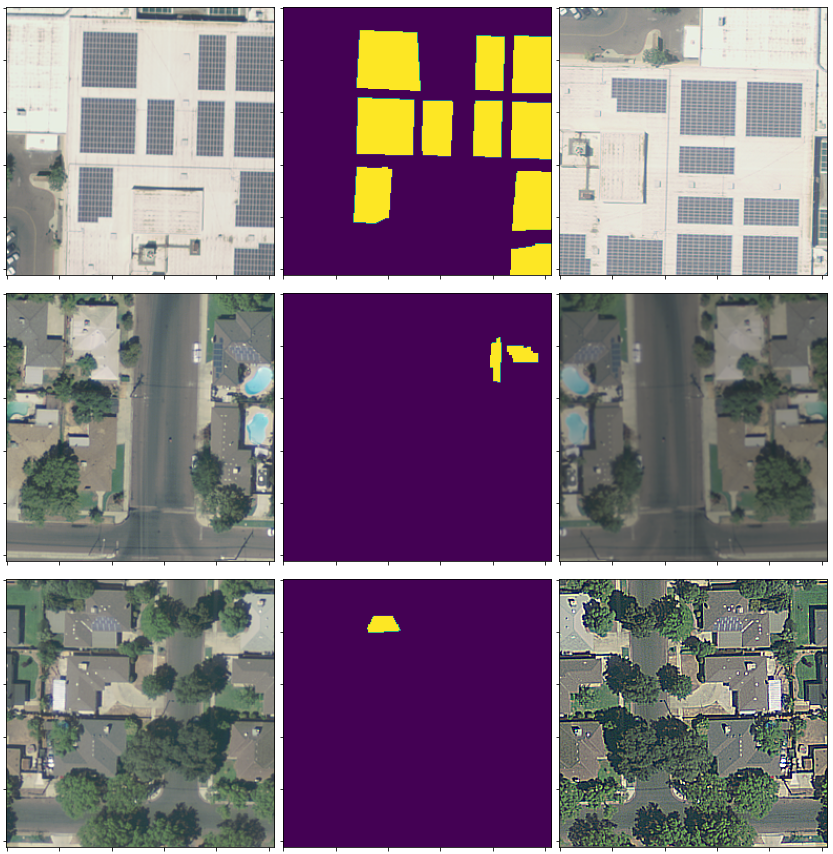
\includegraphics[width=\columnwidth]{resources/png/sample.png}
    \caption{Californian dataset sample with their masks (center) and some random augmentations (right).}
    \label{fig:augment_masks}
\end{figure}

Furthermore, we have annotated, using the \enquote{VGG Image Annotator} \cite{dutta2019vgg}, 661 WalOnMap images ($512 \times 512$) to \emph{fine tune} our networks after having trained them on the Californian dataset.

\subsection{Metrics}
\label{subsec:metrics}

In \cite{yu2018deepsolar}, \cite{malof2016automatic} and \cite{malof2016deep}, the metrics used to characterize the \emph{detection} performances are the \emph{precision} and \emph{recall}. Precision measures the ratio of correct predictions among positive predictions. Recall measures the ratio of correct predictions among positive instances. However, conversely to these papers, we don't have \emph{detection} networks; strictly speaking. Therefore, in order to compare our \emph{detection} capabilities, we perform a \enquote{matching} between the contours of the target mask and those of the output mask. Basically, a target and an output contours match if their intersection is not empty, even barely. It should be noted that very small contours in the output mask are not considered as positive predictions.

For the size estimation, \emph{i.e} segmentation, we use the precision and recall metrics as well, but at the pixel level and only for predictions that we know are correct (true positive detection).

Furthermore, the authors of DeepSolar \cite{yu2018deepsolar}, introduced the \emph{mean relative error} (MRE) as
\begin{equation}
    \text{MRE} = 1 - \frac{\sum_{\text{true positive}} \text{estimated area}}{\sum_{\text{true positive}} \text{true area}}
\end{equation}
which we also compute for the sake of comparison.

Finally, our measures of precision and recall are dependant on a \emph{
threshold} parameter. Therefore, it is sometimes preferred to use the \emph{average precision} instead, which can be visualized as the area under the \emph{precision-recall} curve. The average precision is the metric we use to compare our models.

\emph{Note.} It should be noted that the threshold is shared for detection and segmentation.

\section{Results} \label{sec:results}

In this section, we present the results of training the implemented networks for 20 epochs on the Californian dataset. In order to assess the uncertainty of our metrics, we perform a \emph{5-fold cross validation}. The principle of $k$-fold cross validation is to divide a training set into $k$ folds and to train $k$ independent models on all folds but one. The latter is the validation fold, while the others are the training folds.

\emph{Note.} A few prediction examples on the Californian dataset are provided in the Appendix \ref{subapp:predictions} as well as additional graphs in the Appendix \ref{subapp:metrics}.

\vspace{1em}

\paragraph{Convergence}
To assess the convergence of our models, we evaluate their loss during the training phase on the training folds. The considered losses depend on the network architecture, as defined in section \ref{subsec:losses}.

\begin{figure}[h]
    \centering
    \vspace{-1em}
    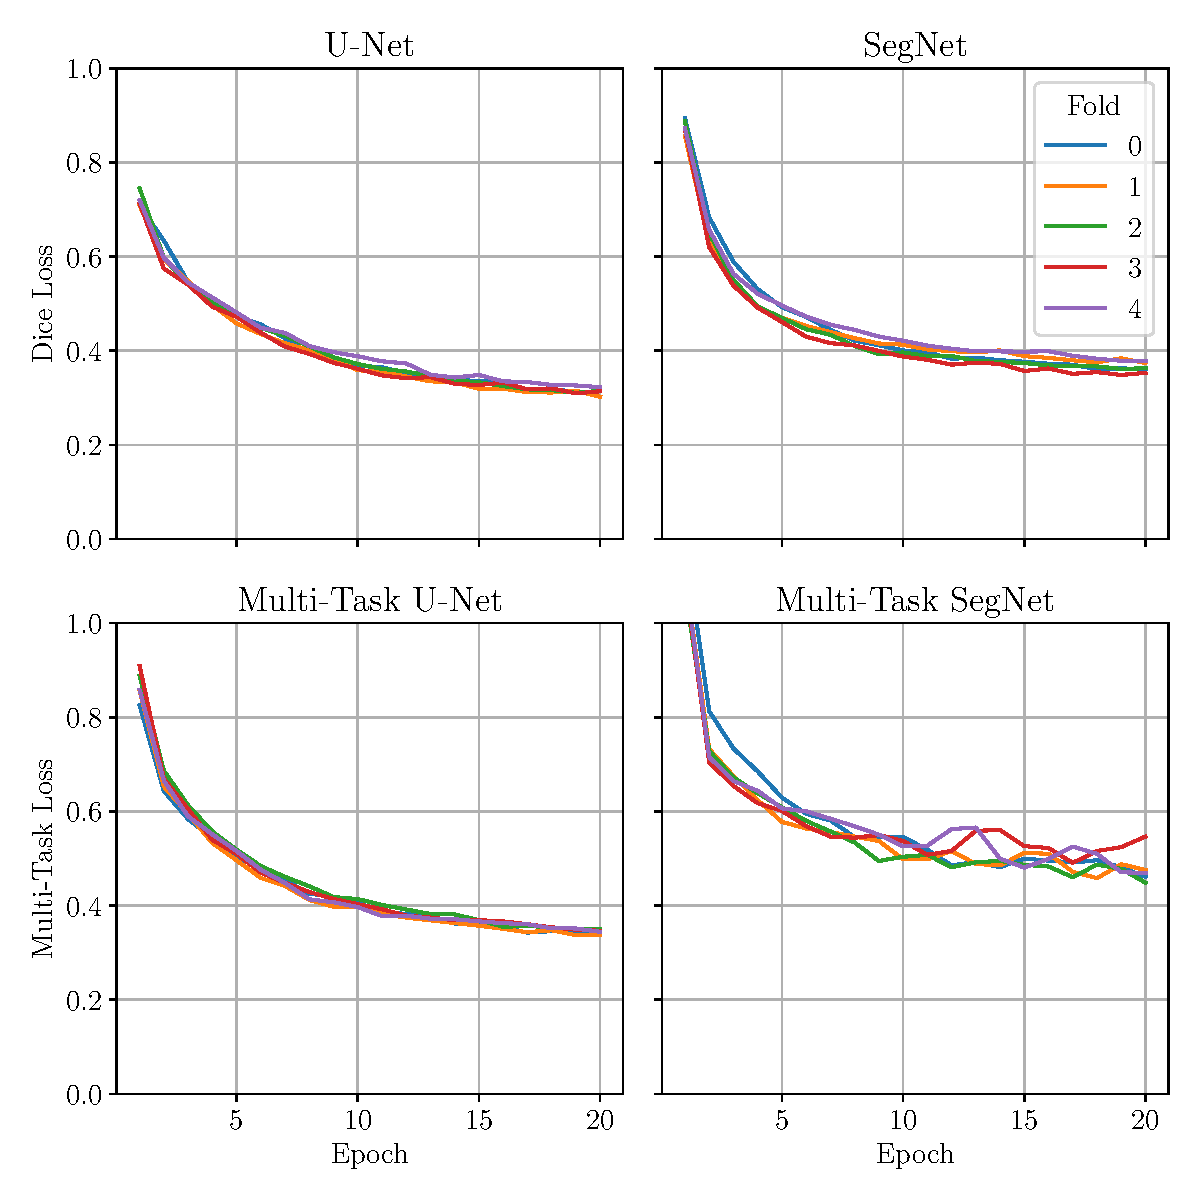
\includegraphics[width=\columnwidth]{resources/pdf/convergence.pdf}
    \vspace{-2em}
    \caption{Mean training losses during 20 epochs. Each color corresponds to a different training-validation folds set.}
    \label{fig:convergence}
\end{figure}

As can be seen from FIG. \ref{fig:convergence}, all four models seem to converge to some fixed value. Convergence looks similar in terms of speed, and the variance w.r.t. the folds looks rather small, which suggests that the folds are representative of the whole dataset. However, both SegNet networks have higher losses and variances than their U-Net counterpart, which means they have more trouble to learn. This would not be surprising as they are also significantly smaller.

Moreover, we can observe that the Multi-Task loss is only slightly over the corresponding Dice Loss, suggesting that the distances are well learnt or that they help learning the mask. That being said, the cross-entropy loss does not take into account the imbalance between the different classes, probably leading to a very low loss thanks to the background class (most negative distance).

\vspace{1em}

\paragraph{Detection}

As mentioned in section \ref{subsec:metrics}, we use precision and recall on the validation fold to assess the \emph{detection} performance of all four models.

\begin{figure}[h]
    \centering
    \vspace{-1em}
    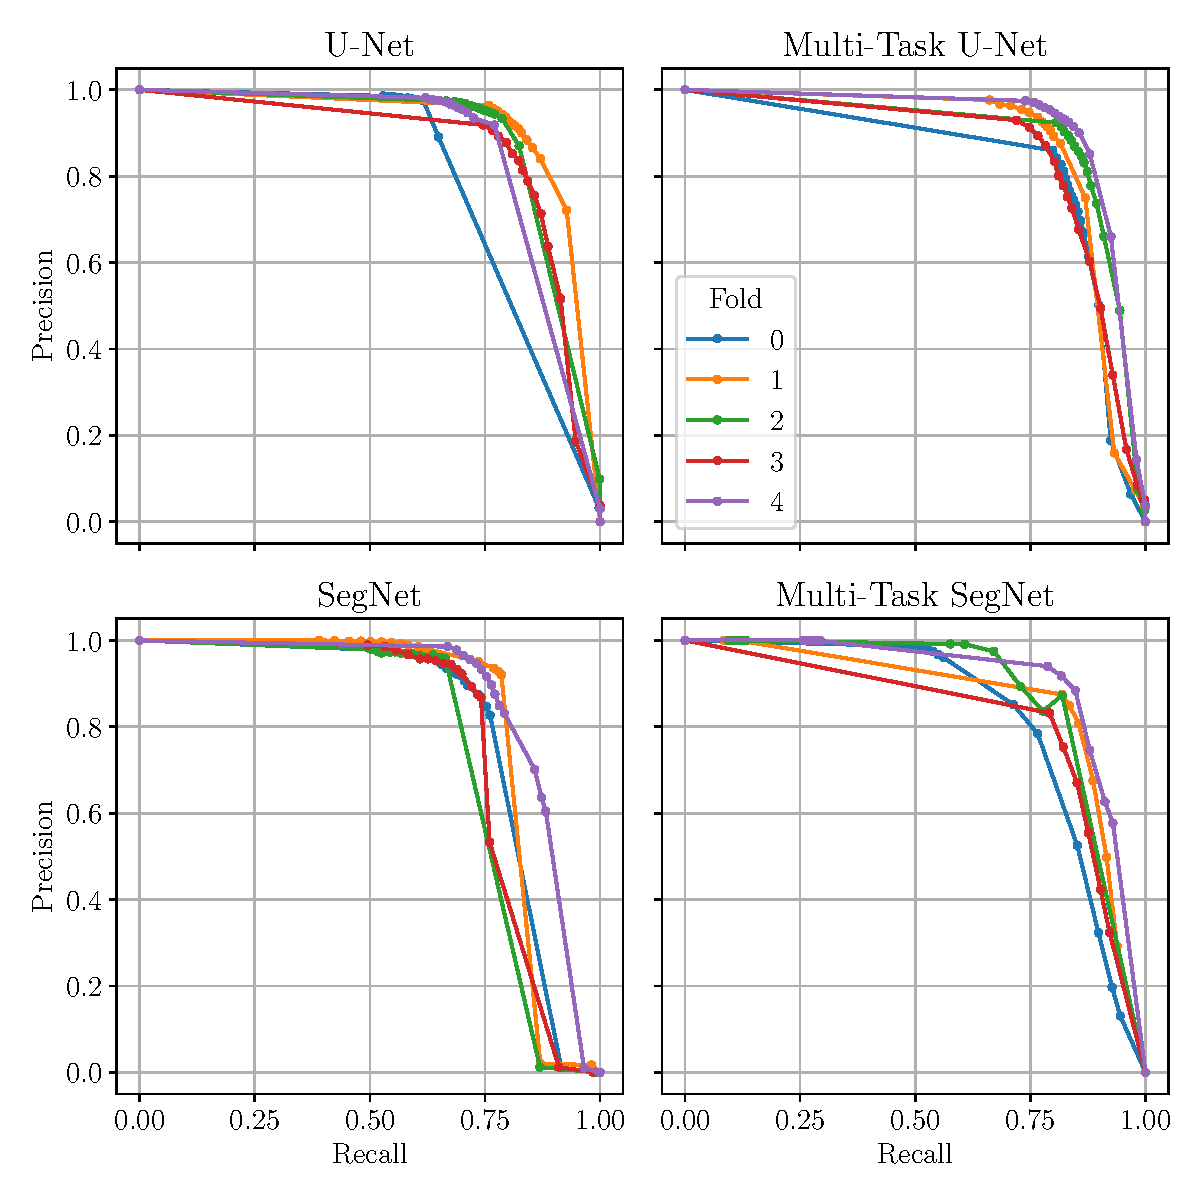
\includegraphics[width=\columnwidth]{resources/pdf/detection_pr.pdf}
    \vspace{-2em}
    \caption{Detection precision and recall of the networks after 20 epochs of training. Each color corresponds to a different training-validation folds set. The thresholds are $0, \num{e-9}, \num{e-8}, \dots, \num{e-1}, 0.5, 1 - \num{e-1}, 1 - \num{e-2}, \dots, 1 - \num{e-9}$ and $1$.}
    \label{fig:detection_pr}
\end{figure}

All models do not perform equivalently in terms of detection, as can be seen from FIG. \ref{fig:detection_pr}. For both U-Net models and SegNet, most precision-recall pairs are located in the up-right corner, meaning that the background and foreground are well segregated; either near 0 or near 1. Furthermore, the curves seem consistent with respect to the fold, especially for Multi-Task U-Net.

Conversely, for Multi-Task SegNet the pairs are mostly located in the up-left corner, reflecting a significant uncertainty in the predictions, which is emphasised by the notable changes of distribution from one fold to the other for the low thresholds. As a consequence, even though the precision recall curves don't necessarily look terrible, it is not actually possible to choose an adequate threshold for this model.

\vspace{1em}

\paragraph{Segmentation}

Based on the true positive detection predictions, we compute the precision and recall of the panel segmentation.

\begin{figure}[h]
    \centering
    \vspace{-1em}
    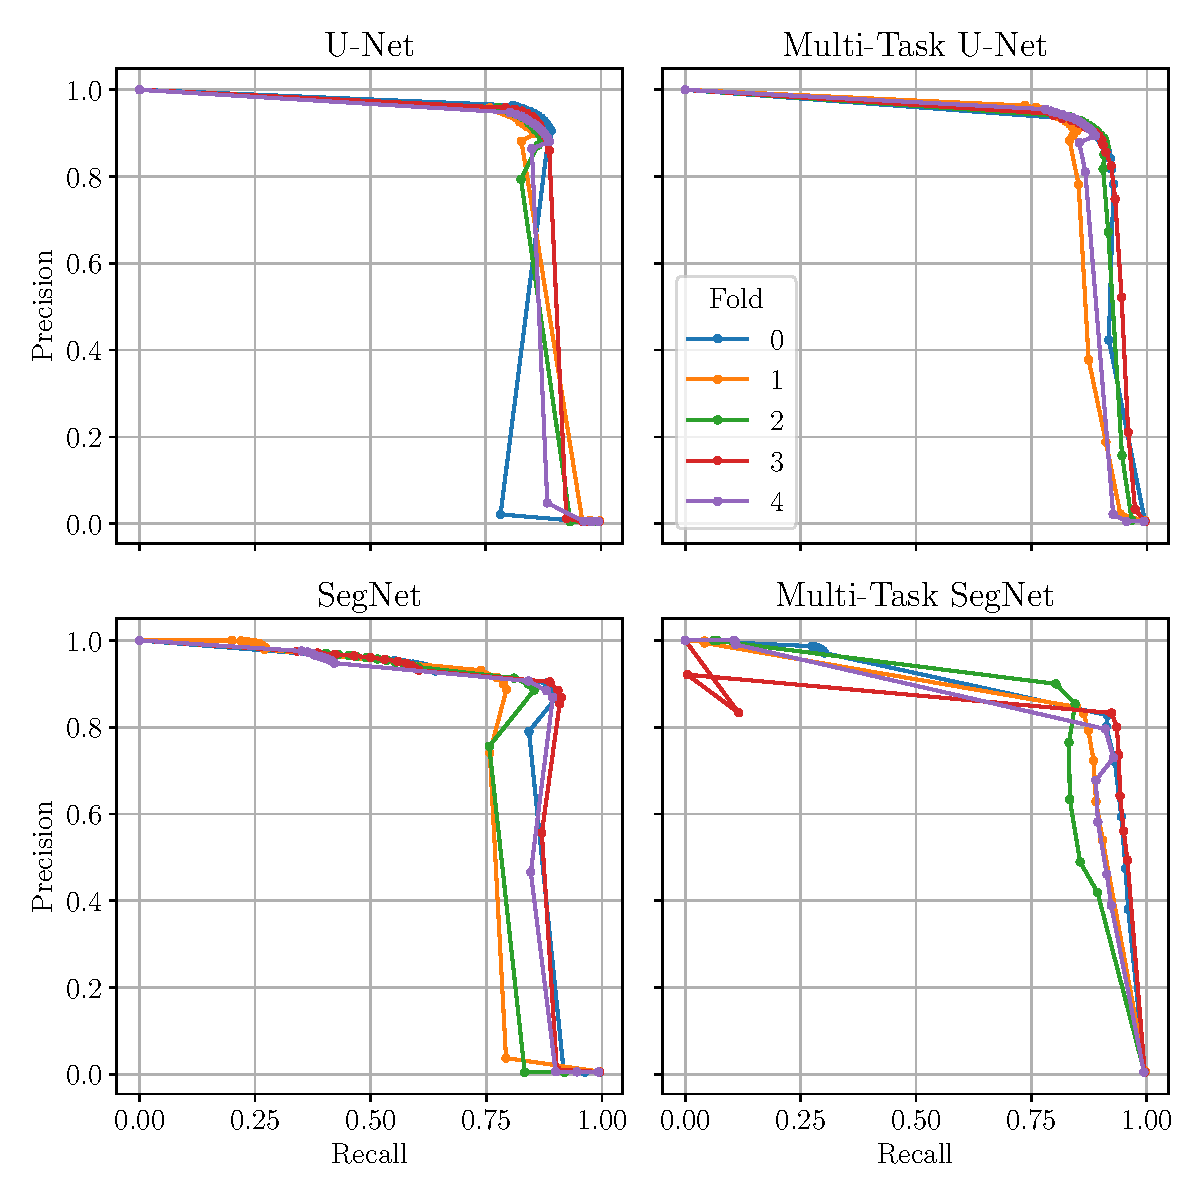
\includegraphics[width=\columnwidth]{resources/pdf/segmentation_pr.pdf}
    \vspace{-2em}
    \caption{Segmentation precision and recall of the networks after 20 epochs of training. Each color corresponds to a different training-validation folds set. The thresholds are the same as in FIG. \ref{fig:detection_pr}.}
    \label{fig:segmentation_pr}
\end{figure}

The results of FIG. \ref{fig:segmentation_pr} show a significant performance difference between U-Net models and SegNet ones. More specifically, the recall of SegNet and Multi-Task Segnet drops rapidly as the threshold increases, which can be clearly observed with FIG. \ref{fig:segmentation_r}. Conversely, U-Net and Multi-Task U-Net are particularly steady w.r.t. to the threshold. These behaviours are emphasized by FIG. \ref{fig:segmentation_mre}.

\begin{figure}[h]
    \centering
    \vspace{-1em}
    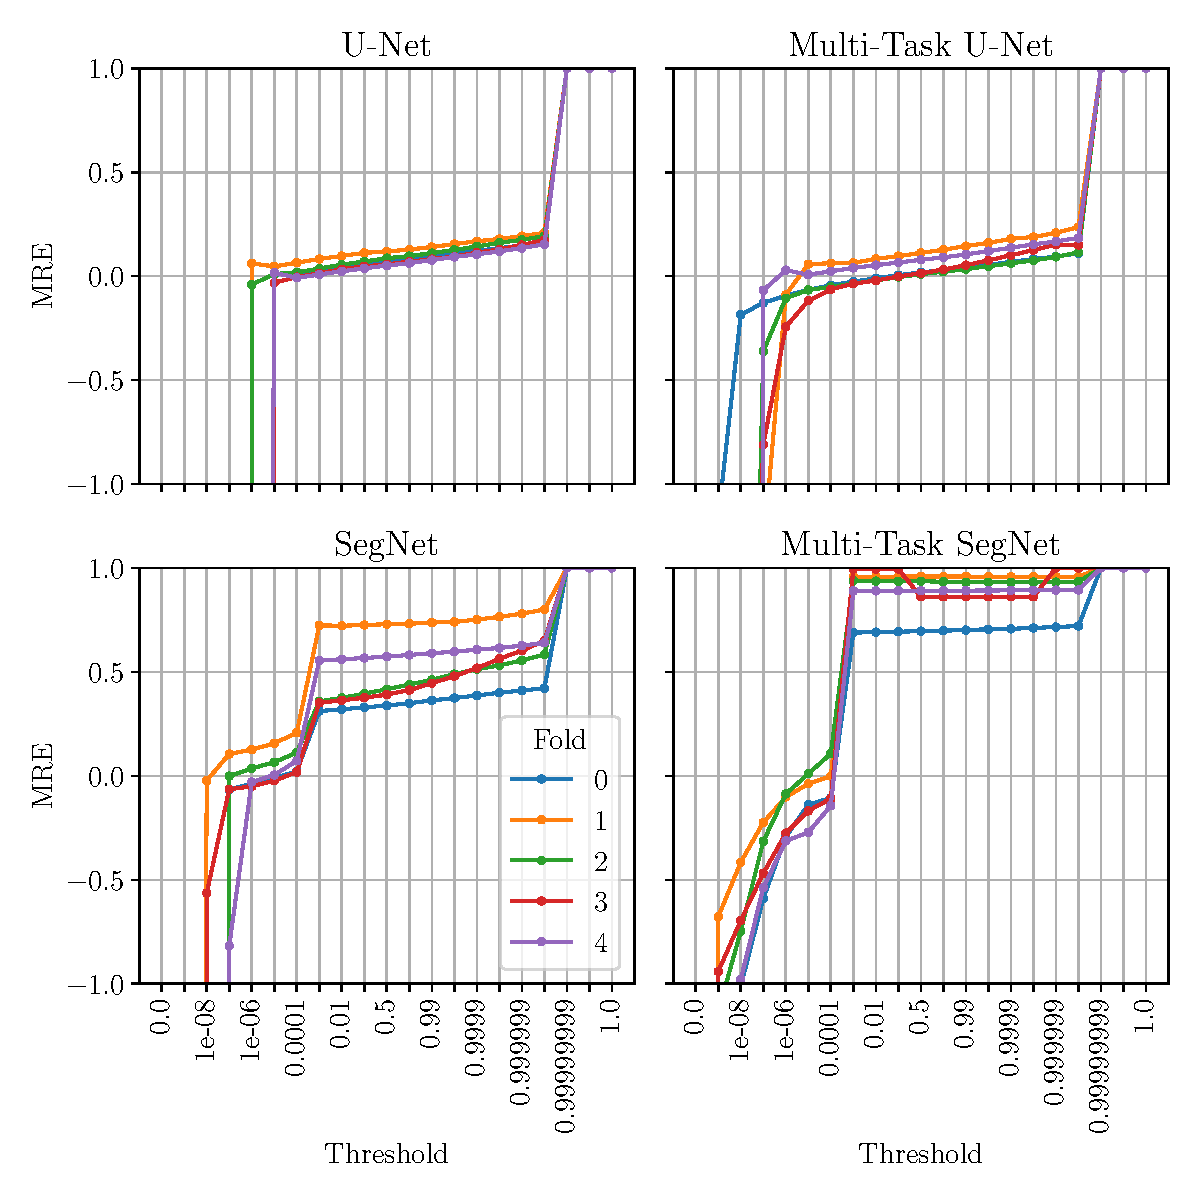
\includegraphics[width=\columnwidth]{resources/pdf/segmentation_mre.pdf}
    \vspace{-2em}
    \caption{Segmentation MRE of the networks after 20 epochs of training, w.r.t. the threshold. Each color corresponds to a different training-validation folds set.}
    \label{fig:segmentation_mre}
\end{figure}

Indeed, we observe that U-Net and Multi-Task U-Net are nearly unbiased (MRE $\simeq$ 0) for the majority of the thresholds while SegNet and Multi-Task SegNet either underestimate or overestimate largely the area.

\vspace{1em}

\paragraph{Comparison}

We estimate the average precision of a model as the mean of its average precision on the different folds.

\begin{table}[h]
    \begin{tabular}{l|c|c}
                      & Detection AP & Segmentation AP \\ \hline
    U-Net             & $0.868 \pm 0.038$ & $0.848 \pm 0.019$ \\ 
    Multi-Task U-Net  & $0.875 \pm 0.030$ & $0.881 \pm 0.020$ \\
    SegNet            & $0.806 \pm 0.039$ & $0.805 \pm 0.039$ \\
    Multi-Task SegNet & $0.858 \pm 0.032$ & $0.848 \pm 0.016$         
    \end{tabular}
    \caption{Average precision of the networks after 20 epochs of training.}
    \label{tab:average_precision}
\end{table}

\begin{figure}[h]
    \centering
    \vspace{-1em}
    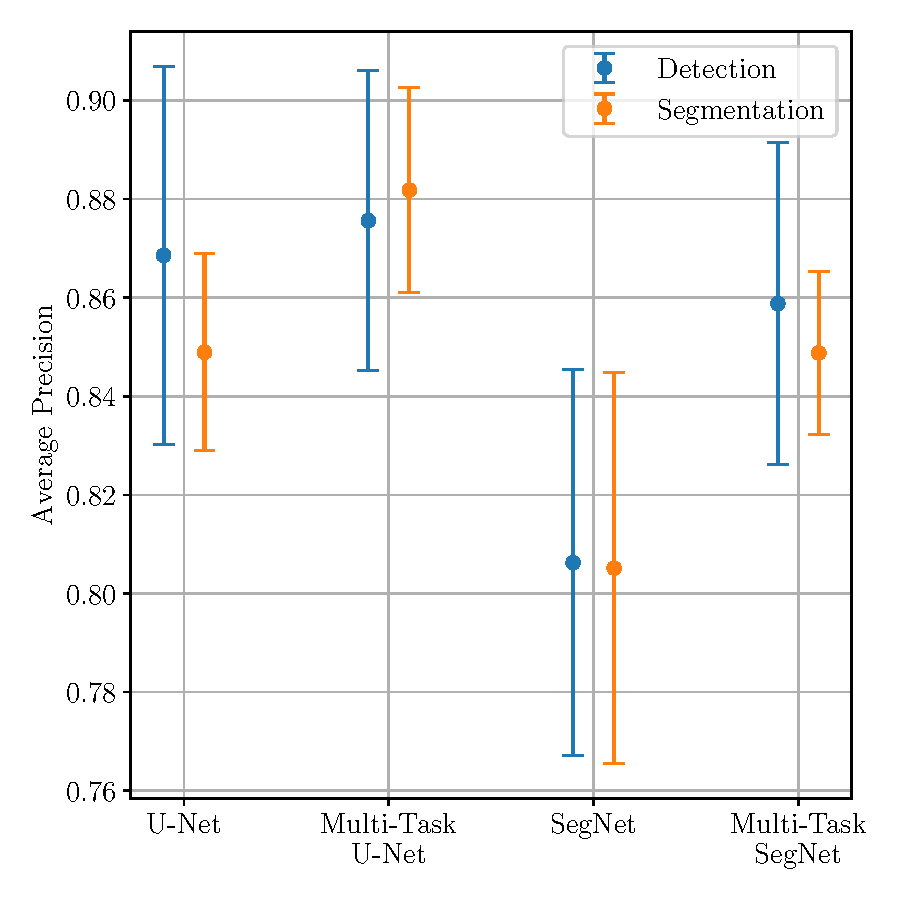
\includegraphics[width=0.75\columnwidth]{resources/pdf/ap.pdf}
    \vspace{-1em}
    \caption{Average precision of the networks after 20 epochs of training.}
    \label{fig:average_precision}
\end{figure}

Our best model is Multi-Task U-Net both in detection and segmentation, reaching above $0.87$ average precision in both tasks. For the rest of this report, we only use this model. Also, we choose a threshold of $0.5$, as it is the most consistent threshold among all folds and as it balances quite well precision and recall.

\begin{table}[h]
    \begin{tabular}{l|c|c}
                               & Metric       & Value \\ \hline
    \multirow{2}{*}{Detection} & Precision    & $0.841 \pm 0.078$ \\ \cline{2-3}
                               & Recall       & $0.826 \pm 0.026$ \\ \hline
    \multirow{3}{*}{Segmentation} & Precision & $0.912 \pm 0.013$ \\ \cline{2-3}
                                  & Recall    & $0.869 \pm 0.027$ \\ \cline{2-3}
                                  & MRE       & $0.046 \pm 0.041$
    \end{tabular}
    
    \caption{Multi-Task U-Net average metrics at $0.5$ threshold.}
    \label{tab:average_precision}
\end{table}

\vspace{1em}

\paragraph{Fine tuning}

As explained in the previous section, the model we wish to apply to WalOnMap images is Multi-Task U-Net. However, even though it was trained for 20 epochs on the Californian dataset with substantial data augmentation\footnote{It should be noted that, to match WalOnMap and California scales, we had to up-scale the latter's images by a factor 2.}, the model didn't generalize well to WalOnMap. Therefore, we fine tune our model for 10 more epochs on the 661 WalOnMap images we annotated.

To better assess the performance boost provided by the fine tuning, we divide the 661 images into 5 folds and perform 5-fold cross validation.

\begin{figure}[h]
    \centering
    \vspace{-1em}
    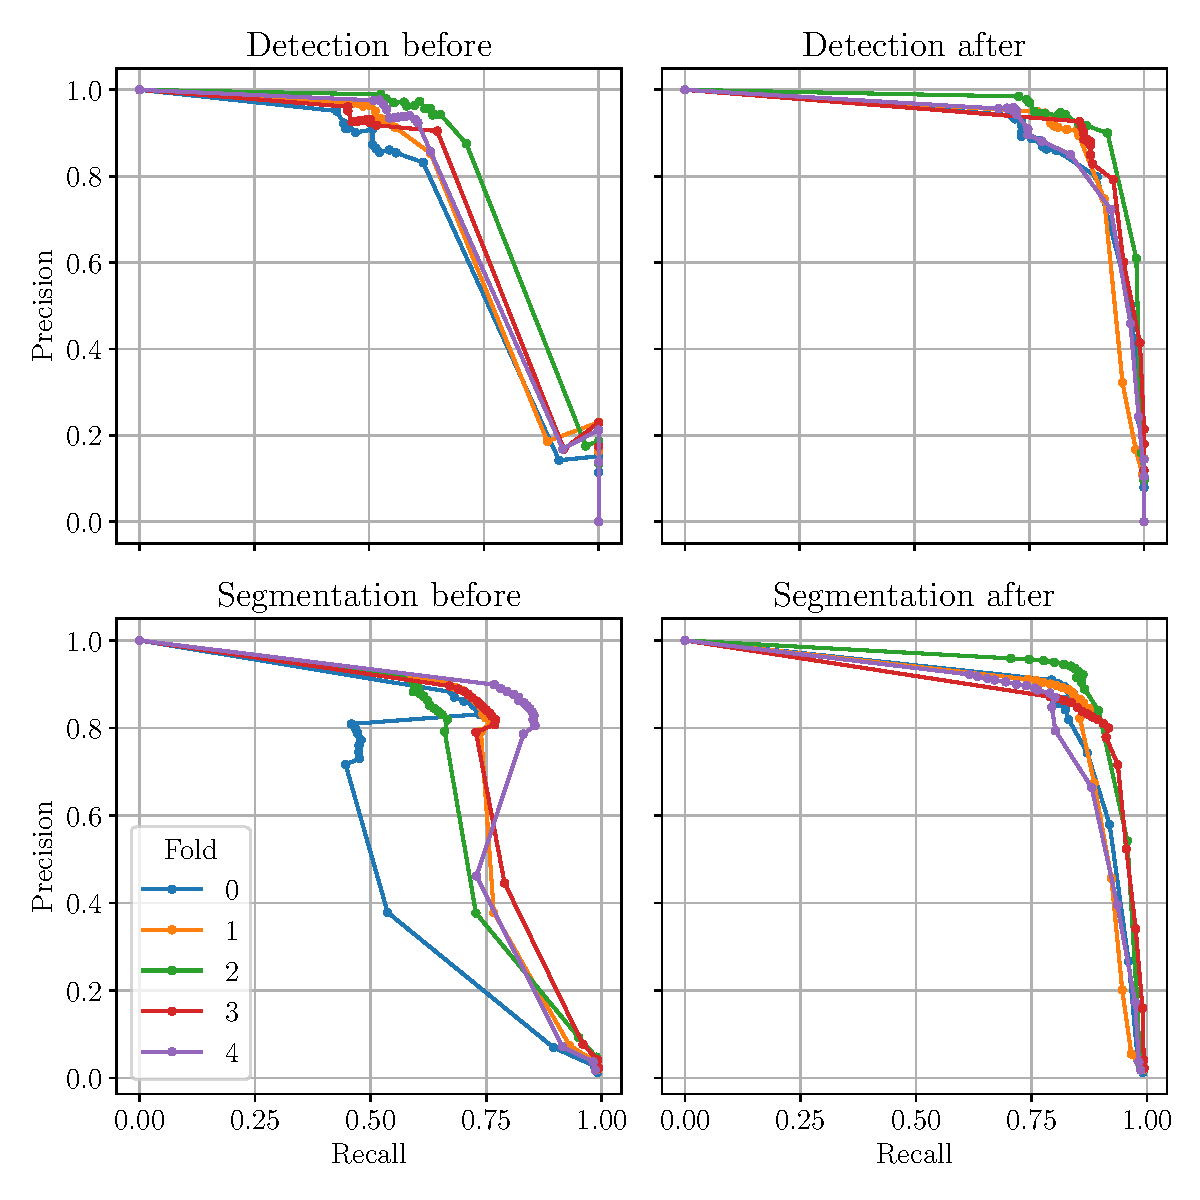
\includegraphics[width=\columnwidth]{resources/pdf/before_after.pdf}
    \vspace{-2em}
    \caption{Detection and segmentation precision and recall before and after $10$ epochs of fine tuning. Each color corresponds to a different training-validation folds set.}
    \label{fig:before_after}
\end{figure}

As one can see in FIG. \ref{fig:before_after} and TABLE \ref{tab:before_after}, the fine tuning improves significantly and consistently the performances of the network both in detection and segmentation.

\begin{table}[h]
    \begin{tabular}{l|c|c}
                       & Detection AP & Segmentation AP \\ \hline
    Before fine-tuning & $0.783 \pm 0.033$ & $0.703 \pm 0.068$ \\ 
    After fine-tuning  & $0.922 \pm 0.018$ & $0.861 \pm 0.019$ \\       
    \end{tabular}
    \caption{Average precision (AP) before and after $10$ epochs of fine tuning.}
    \label{tab:before_after}
\end{table}

Finally, the model was fine tuned with all $661$ images and used to detect the PV installations in the Province of Liège. The result is showcased as an interactive map at \texttt{\href{https://francois-rozet.github.io/adopptrs/}{https://francois-rozet.github.io/adopptrs/}}.

\section{Discussion} \label{sec:discussion}

Overall, we are satisfied by our results. With a detection precision of $0.841$ and a recall of $0.826$, if we are still far from DeepSolar \cite{yu2018deepsolar} performances ($0.934$ precision and $0.895$ recall), we actually outperform significantly Malof et al. \cite{malof2016deep} detector ($0.72$ precision and $0.8$ recall).

However, it should be noted that DeepSolar's dataset is quite different from ours, therefore the comparison isn't very relevant. Furthermore, both DeepSolar and Malof et al. implemented models with the primary purpose of detecting the panels while, in our case, detection is kind of a \emph{by-product} of the segmentation. Therefore, our results are all the more respectable.

Concerning the segmentation, on average, our final model underestimates slightly ($\SI{4.6}{\percent}$ MRE) the size of the PV arrays. However, as is mentioned in the Appendix \ref{subapp:predictions}, some annotations of the Californian dataset are inaccurate which could lead to a biased metric.

From a broader perspective, it should be emphasized that, separately, the detection and segmentation metrics do not necessarily reflect the actual behaviour of the models as, in a real use-case, these errors would normally add up.

Another point to highlight is that, in this project, we focus mainly on the architecture of the networks, while barely touching to the training hyper-parameters. Also, we only trained our networks for 20 epochs\footnote{Initially, we had not implemented the cross validation. But we realized, quite late, that error bars were asked. Therefore, we started new training jobs, but we did not have the time for more than 20 epochs.}, which might be not enough to learn the task. If we were to continue this project, further investigation of the training procedure would certainly be a priority.

Also, if we decided early on to use Batch Normalization and Data Augmentation, we actually never measured quantitatively the influence they had on our models. This is also a point we should investigate in hypothetical future works.

In addition, when we used our final model to detect all PV installations in the Province of Liège, if most panels were accurately detected and segmented, we noticed qualitatively that a lot of shadows and canopies were misleadingly predicted as PV panels. We don't believe it to be due to the network itself, but rather to the low number and variety of images we hand-annotated. The most obvious way to improve our results would be to annotate more images, which we unfortunately had not the time to do.

Finally, initially and for most of the project, we were only considering the images surrounding the annotations (cf. section \ref{subsec:augmentation}) for both training and validation. Obviously, we obtained very good results but they were extremely biased and did not reflect in other tests we made, which gave us terrible headaches. If there is something we have learned with this project, it is that we should check very carefully and \emph{from the start} that our training and, most importantly, validation procedures are free of bias.

% ==============================================================================

\bibliographystyle{ieeetr}
\bibliography{resources/bibliography.bib}

\clearpage

\appendix

\section{Figures} \label{app:figures}

\subsection{Metrics} \label{subapp:metrics}

\begin{figure}[h]
    \centering
    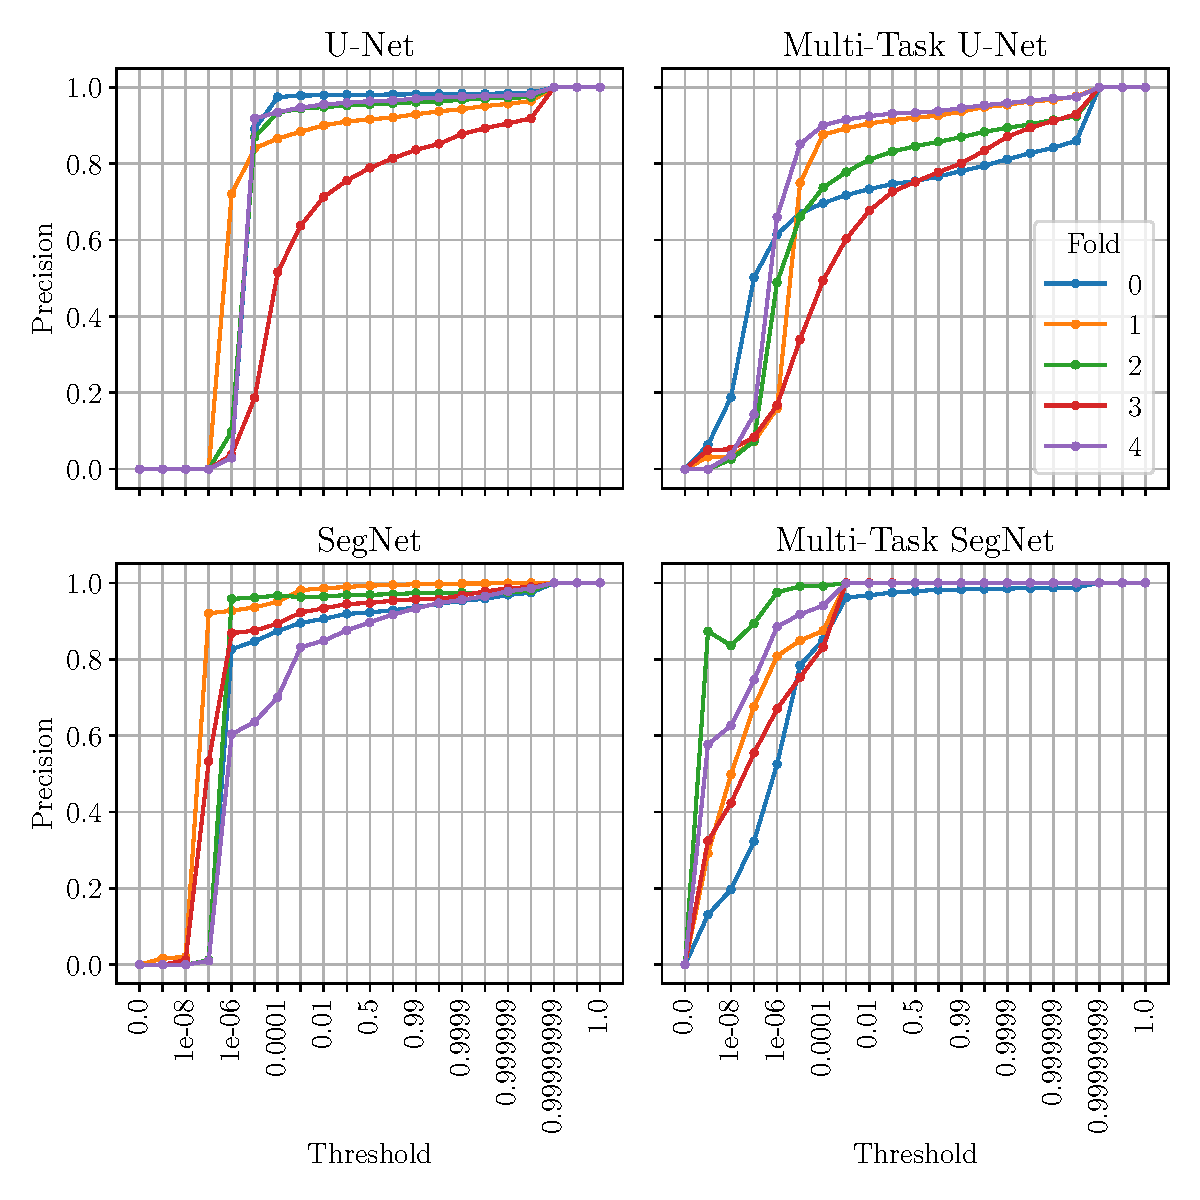
\includegraphics[width=\columnwidth]{resources/pdf/detection_p.pdf}
    \caption{Detection precision w.r.t. the threshold after 20 epochs of training.}
    \label{fig:detection_p}
\end{figure}

\begin{figure}[h]
    \centering
    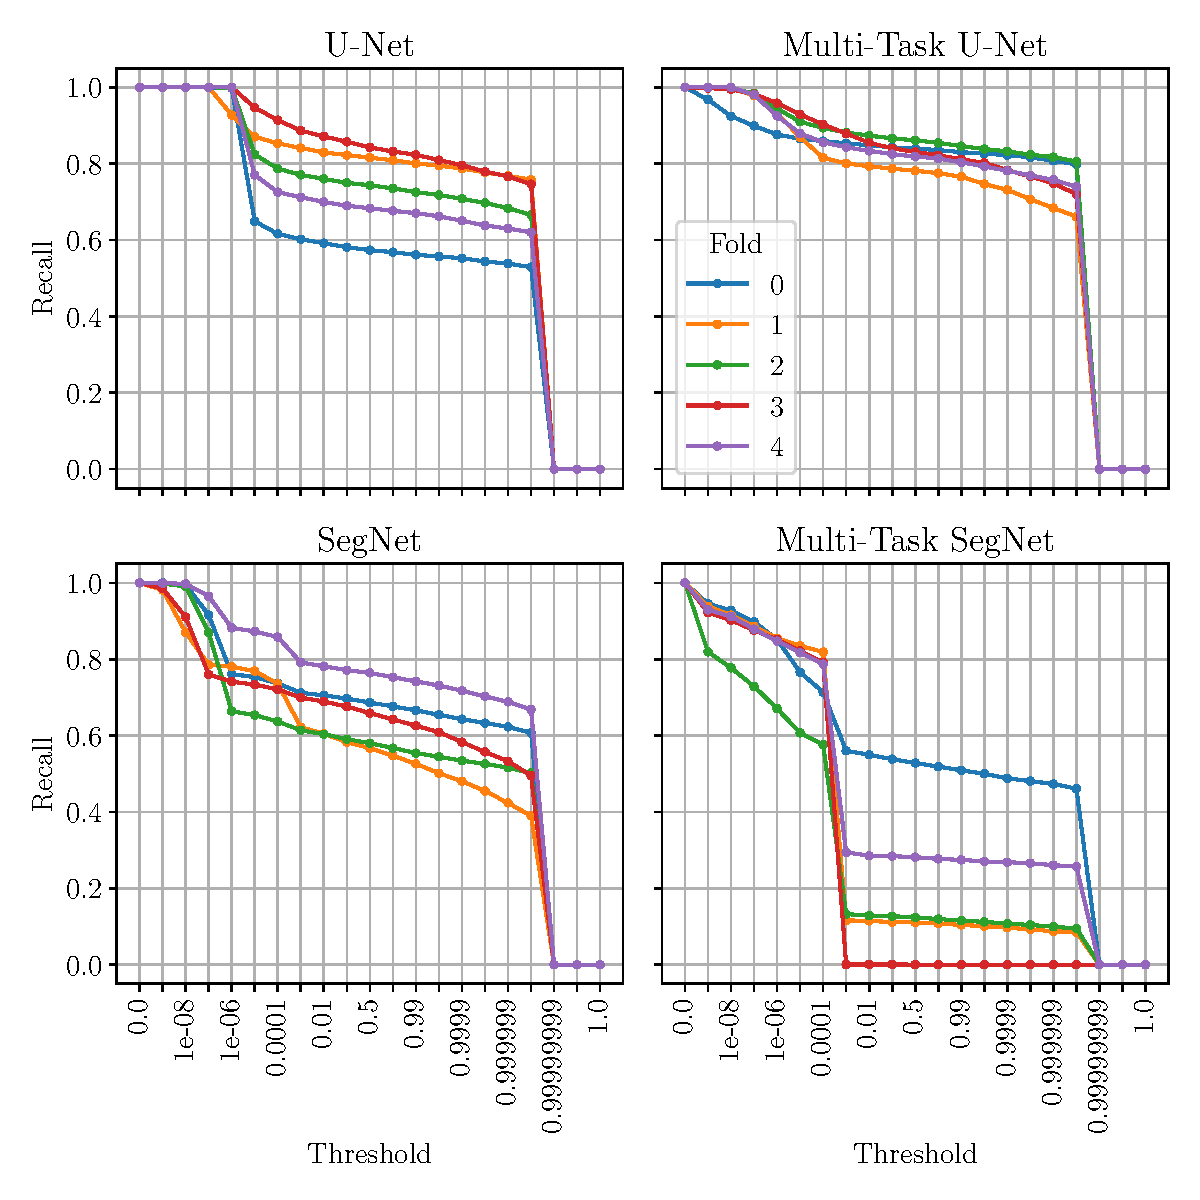
\includegraphics[width=\columnwidth]{resources/pdf/detection_r.pdf}
    \caption{Detection recall w.r.t. the threshold after 20 epochs of training.}
    \label{fig:detection_r}
\end{figure}

\begin{figure}[h]
    \centering
    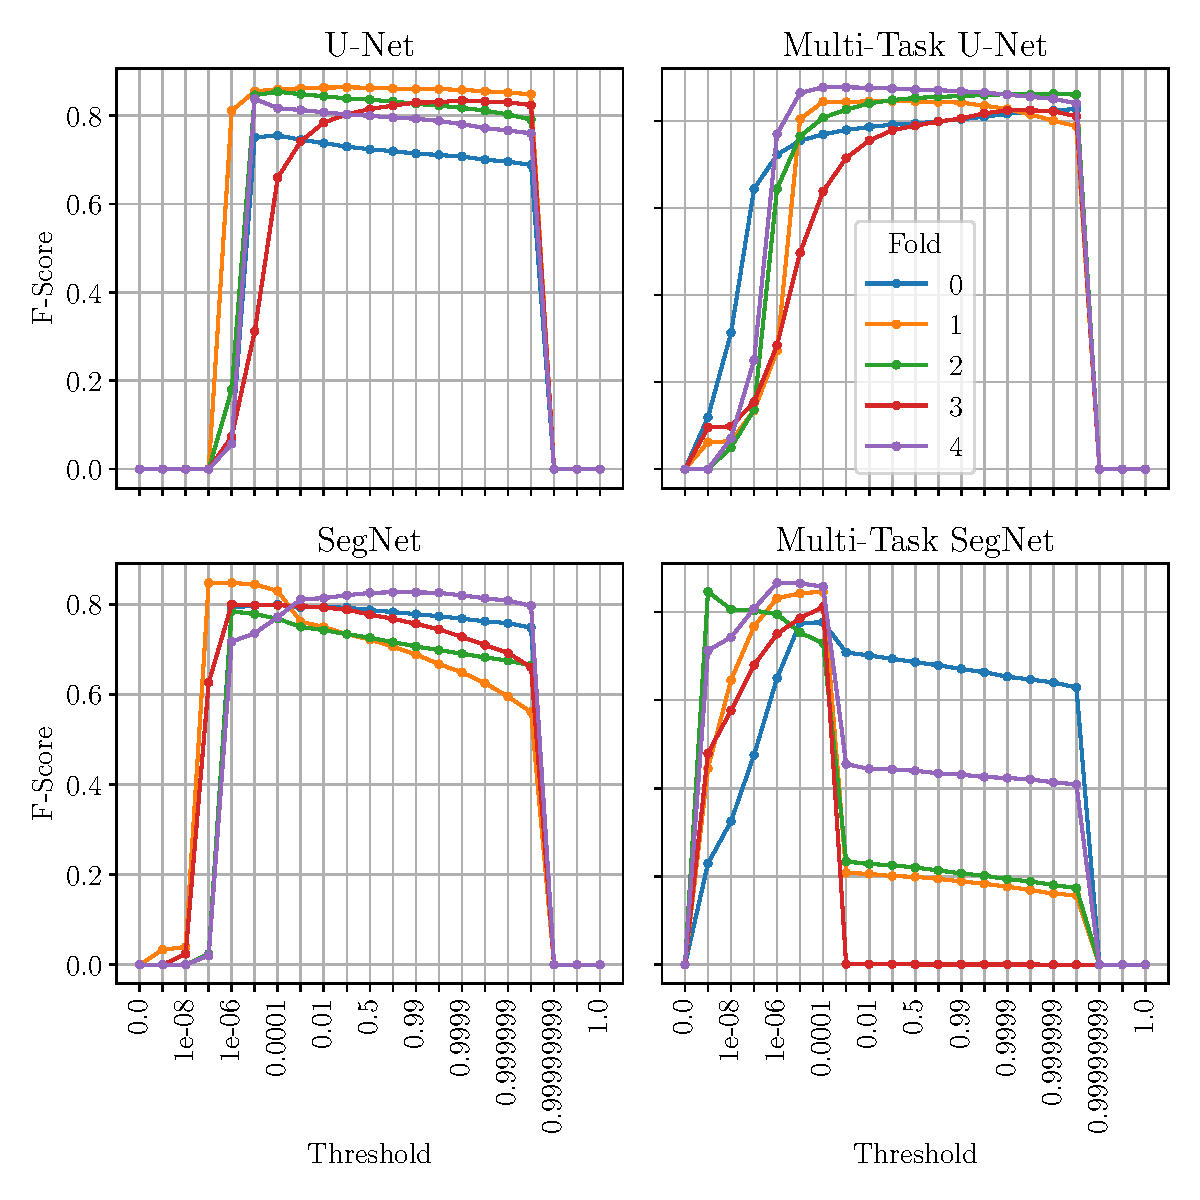
\includegraphics[width=\columnwidth]{resources/pdf/detection_f.pdf}
    \caption{Detection F-Score w.r.t. the threshold after 20 epochs of training.}
    \label{fig:detection_f}
\end{figure}

\begin{figure}[h]
    \centering
    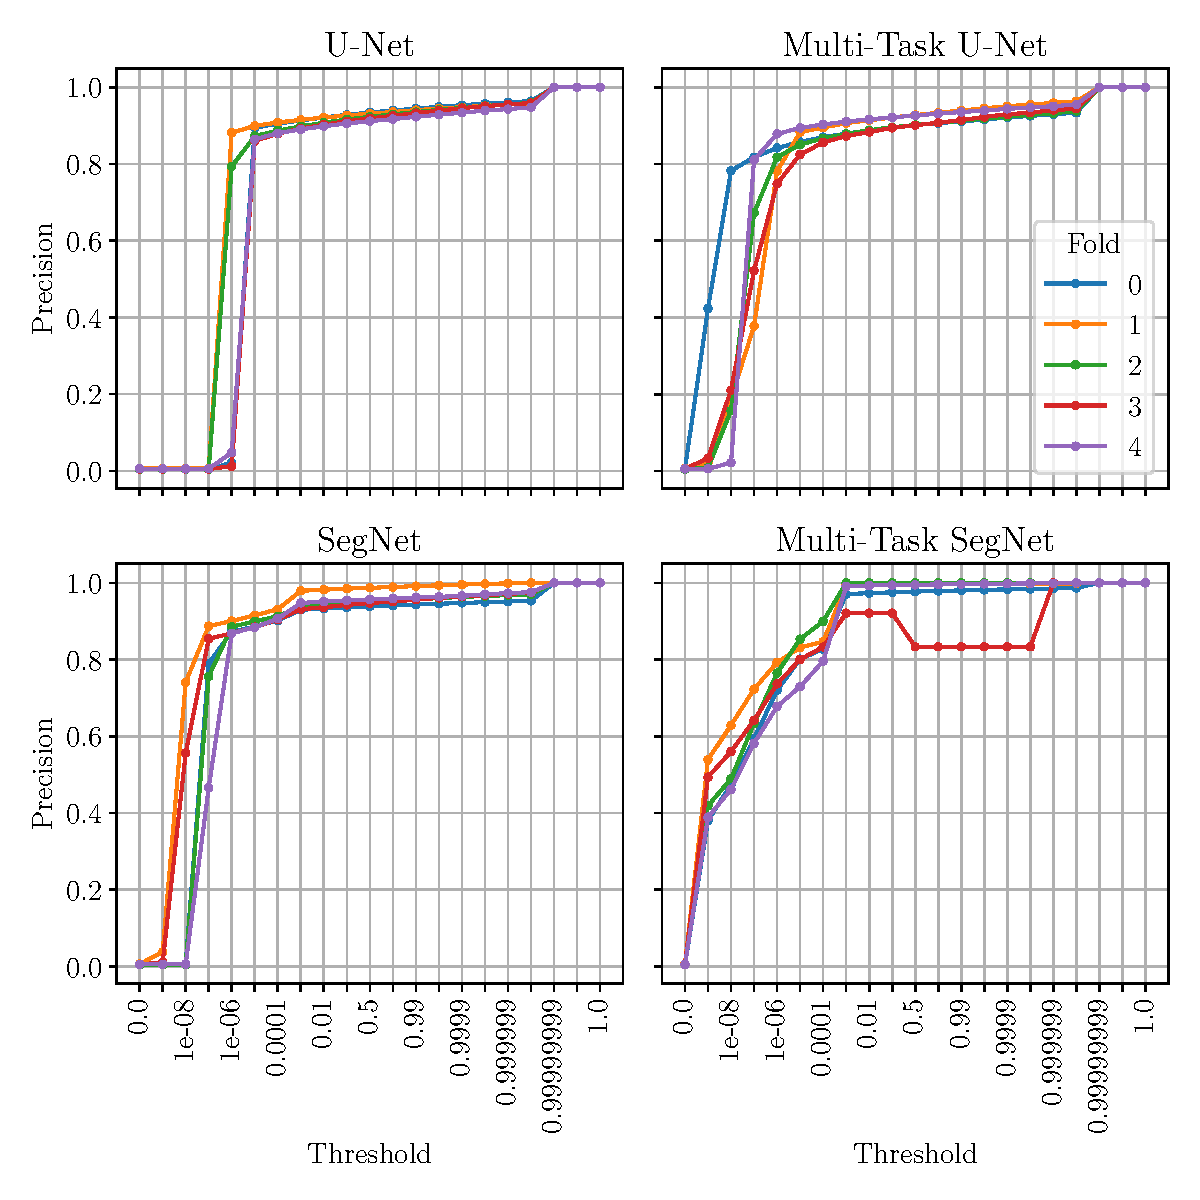
\includegraphics[width=\columnwidth]{resources/pdf/segmentation_p.pdf}
    \caption{Segmentation precision w.r.t. the threshold after 20 epochs of training.}
    \label{fig:segmentation_p}
\end{figure}

\begin{figure}[h]
    \centering
    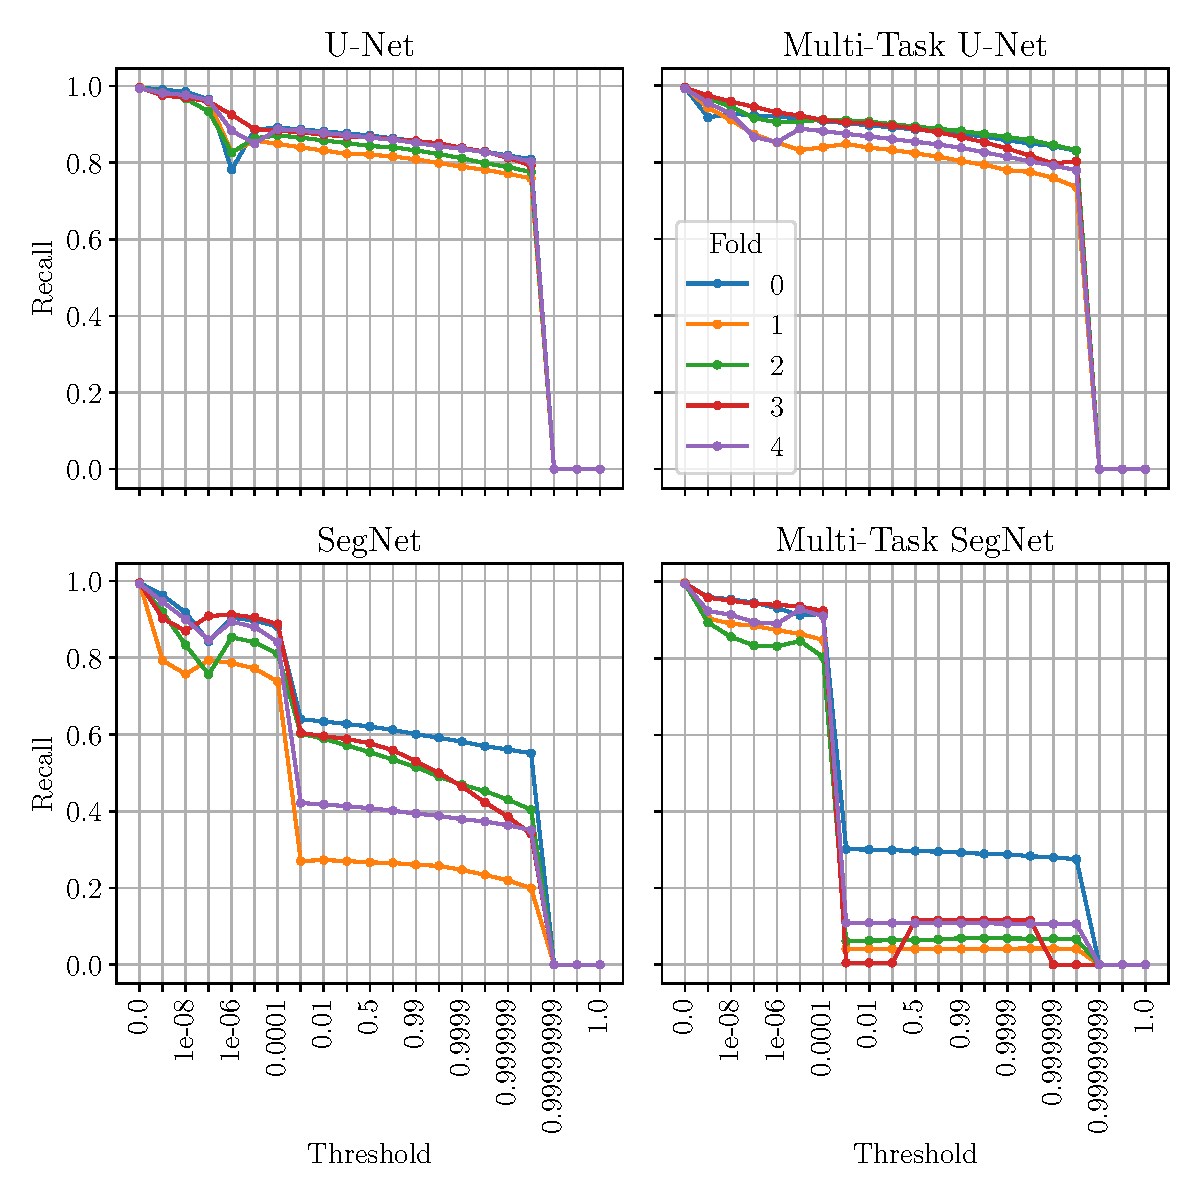
\includegraphics[width=\columnwidth]{resources/pdf/segmentation_r.pdf}
    \caption{Segmentation recall w.r.t. the threshold after 20 epochs of training.}
    \label{fig:segmentation_r}
\end{figure}

\begin{figure}[h]
    \centering
    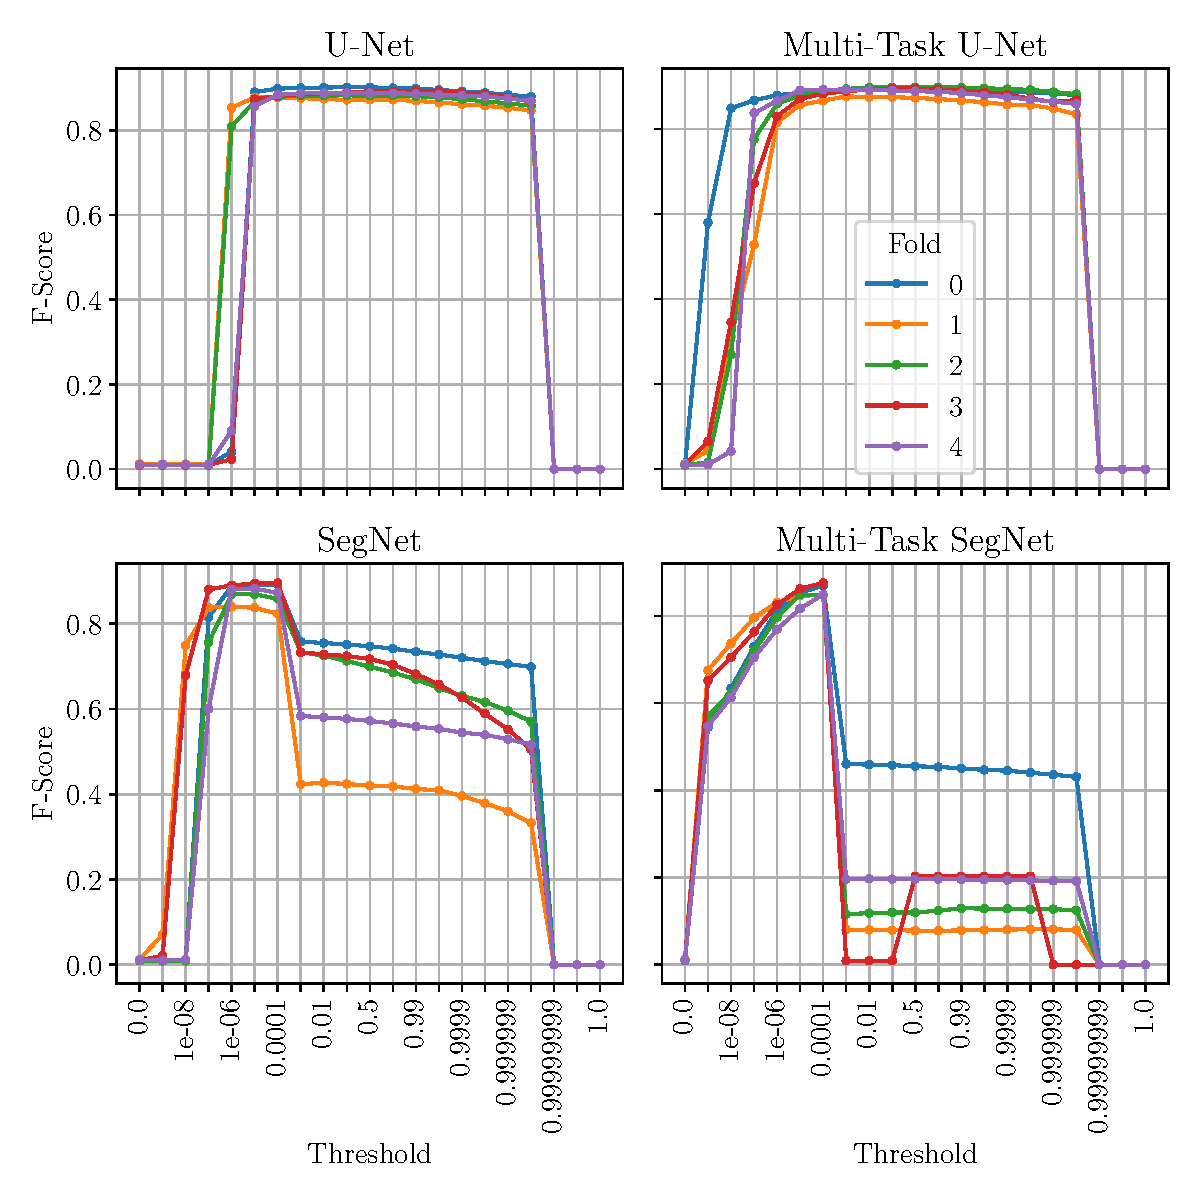
\includegraphics[width=\columnwidth]{resources/pdf/segmentation_f.pdf}
    \caption{Segmentation F-Score w.r.t. the threshold after 20 epochs of training.}
    \label{fig:segmentation_f}
\end{figure}

\clearpage

\subsection{Prediction examples} \label{subapp:predictions}

In this section, a few predictions on positive images are presented. The images were chosen within the fold $1$ and so as to cover a fair variety of cases.

It should be noted that their distribution is \emph{not} respected. In each of the following figures, each column is composed of a raw image, its mask and the predictions of, in this order, the U-Net, Multi-Task U-Net, SegNet and Multi-Task SegNet networks.

\begin{figure}[h]
    \centering
    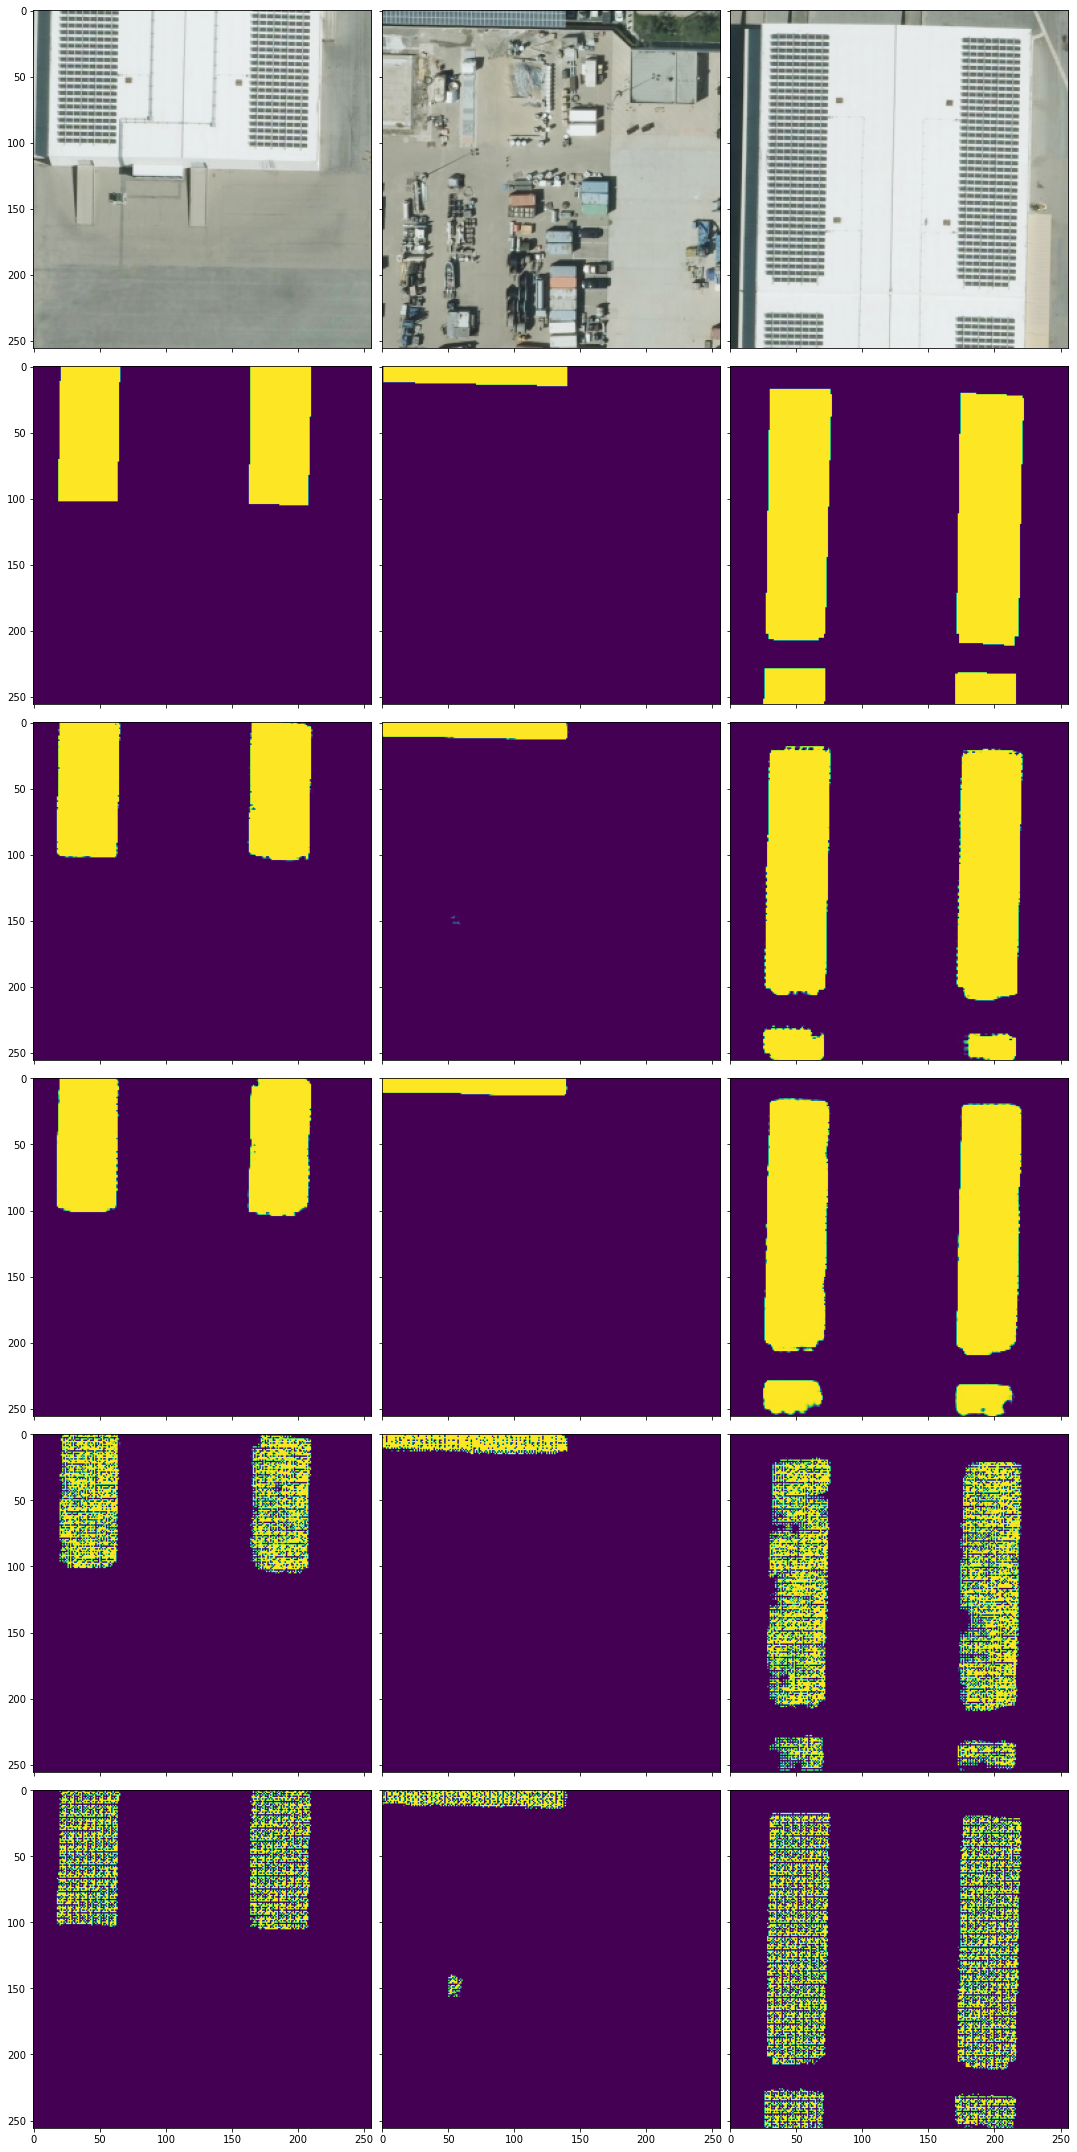
\includegraphics[width=\columnwidth]{resources/png/easy.png}
    \caption{Sample of easy predictions.}
    \label{fig:easy_sample}
\end{figure}

In FIG. \ref{fig:easy_sample}, the four networks detect accurately the panels. However, where U-Net and Multi-Task U-Net are barely hesitant, SegNet and Multi-Task SegNet show a lot of uncertainty. It is actually the case for every prediction. In order to improve the predictions, we could have considered the \emph{closing} operation to merge nearby spots together.

\begin{figure}[h]
    \centering
    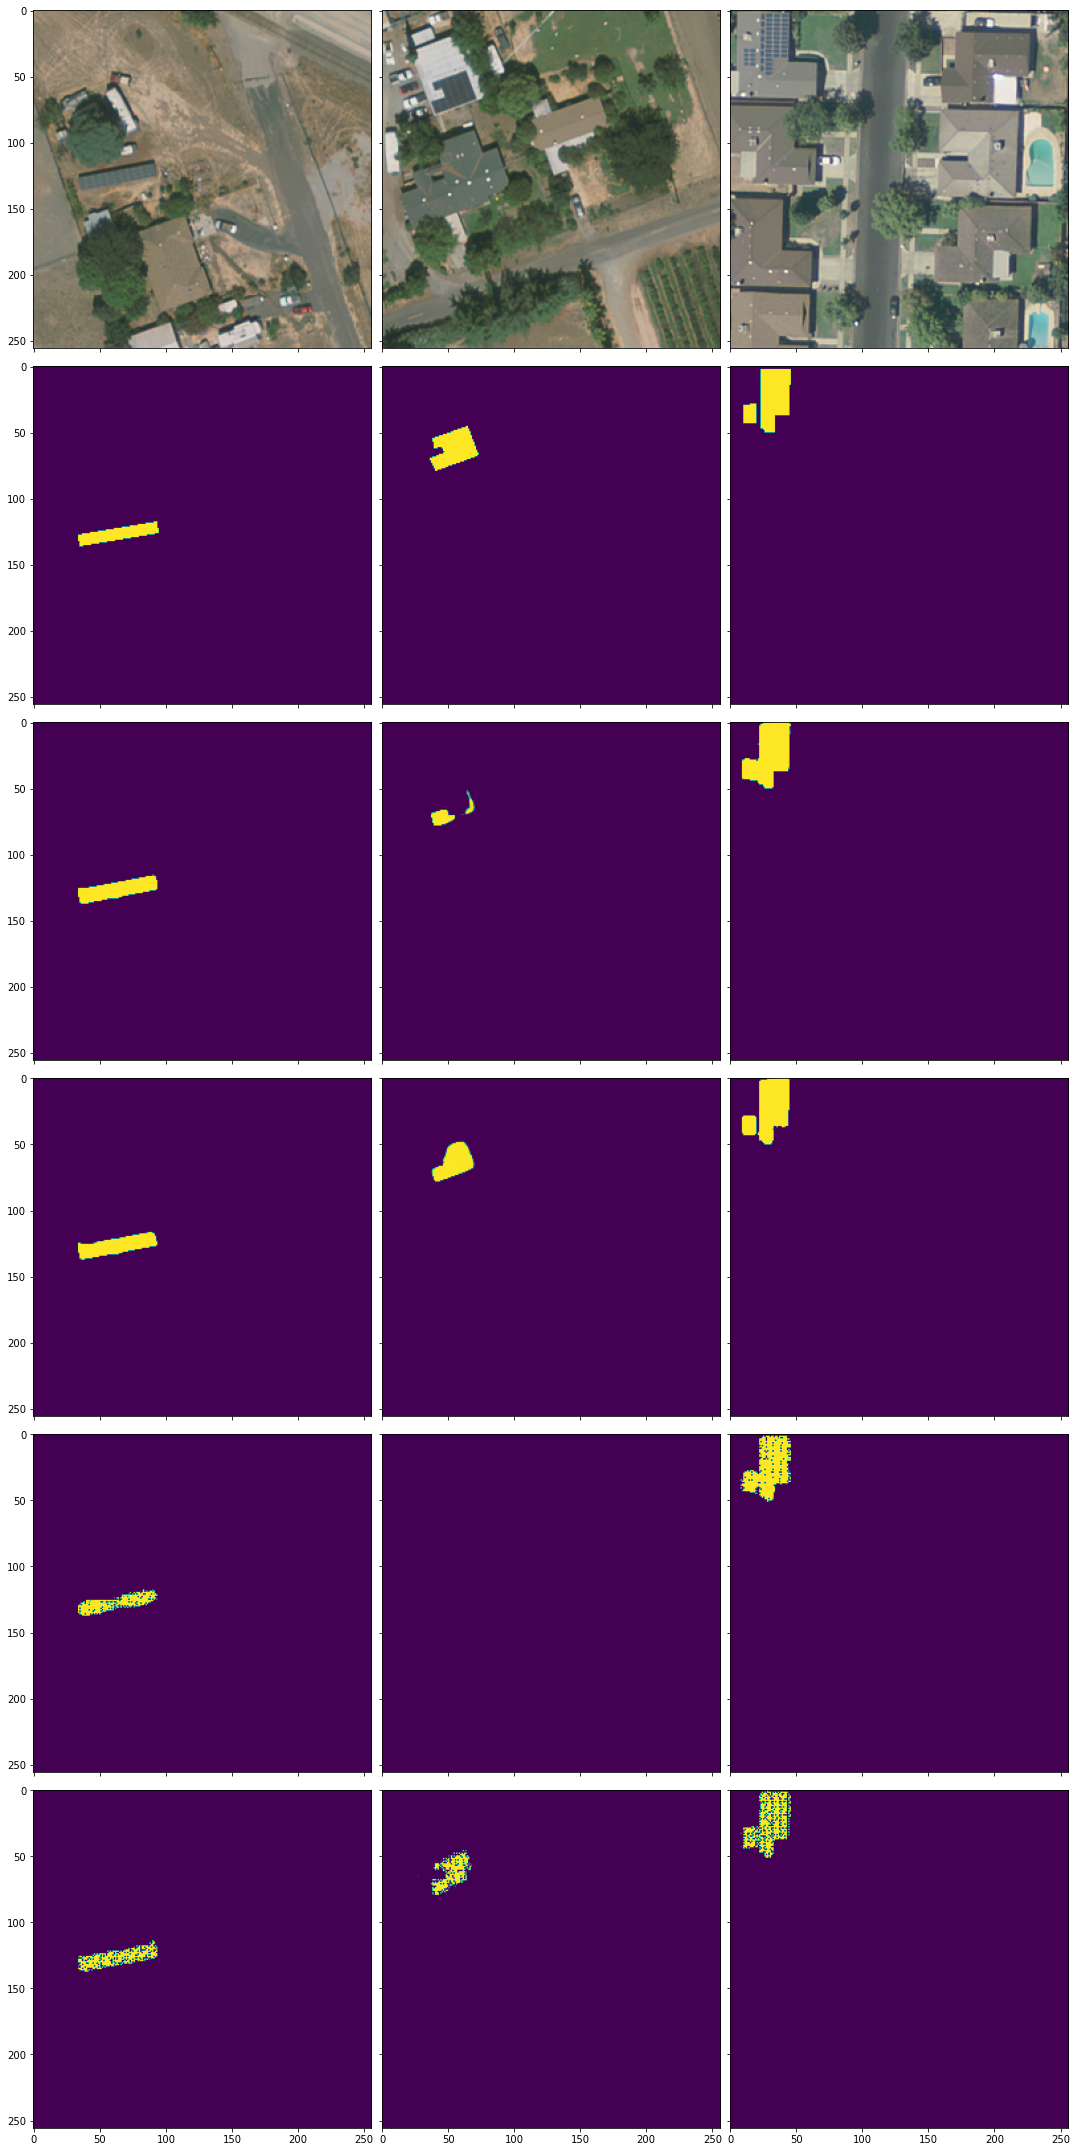
\includegraphics[width=\columnwidth]{resources/png/good.png}
    \caption{Sample of average predictions.}
    \label{fig:average_sample_1}
\end{figure}

In FIG. \ref{fig:average_sample_1}, it appears that Multi-Task U-Net delimits better the boundaries than U-Net, especially for the third image where it successfully differentiates the two sub-arrays.

\begin{figure}[h]
    \centering
    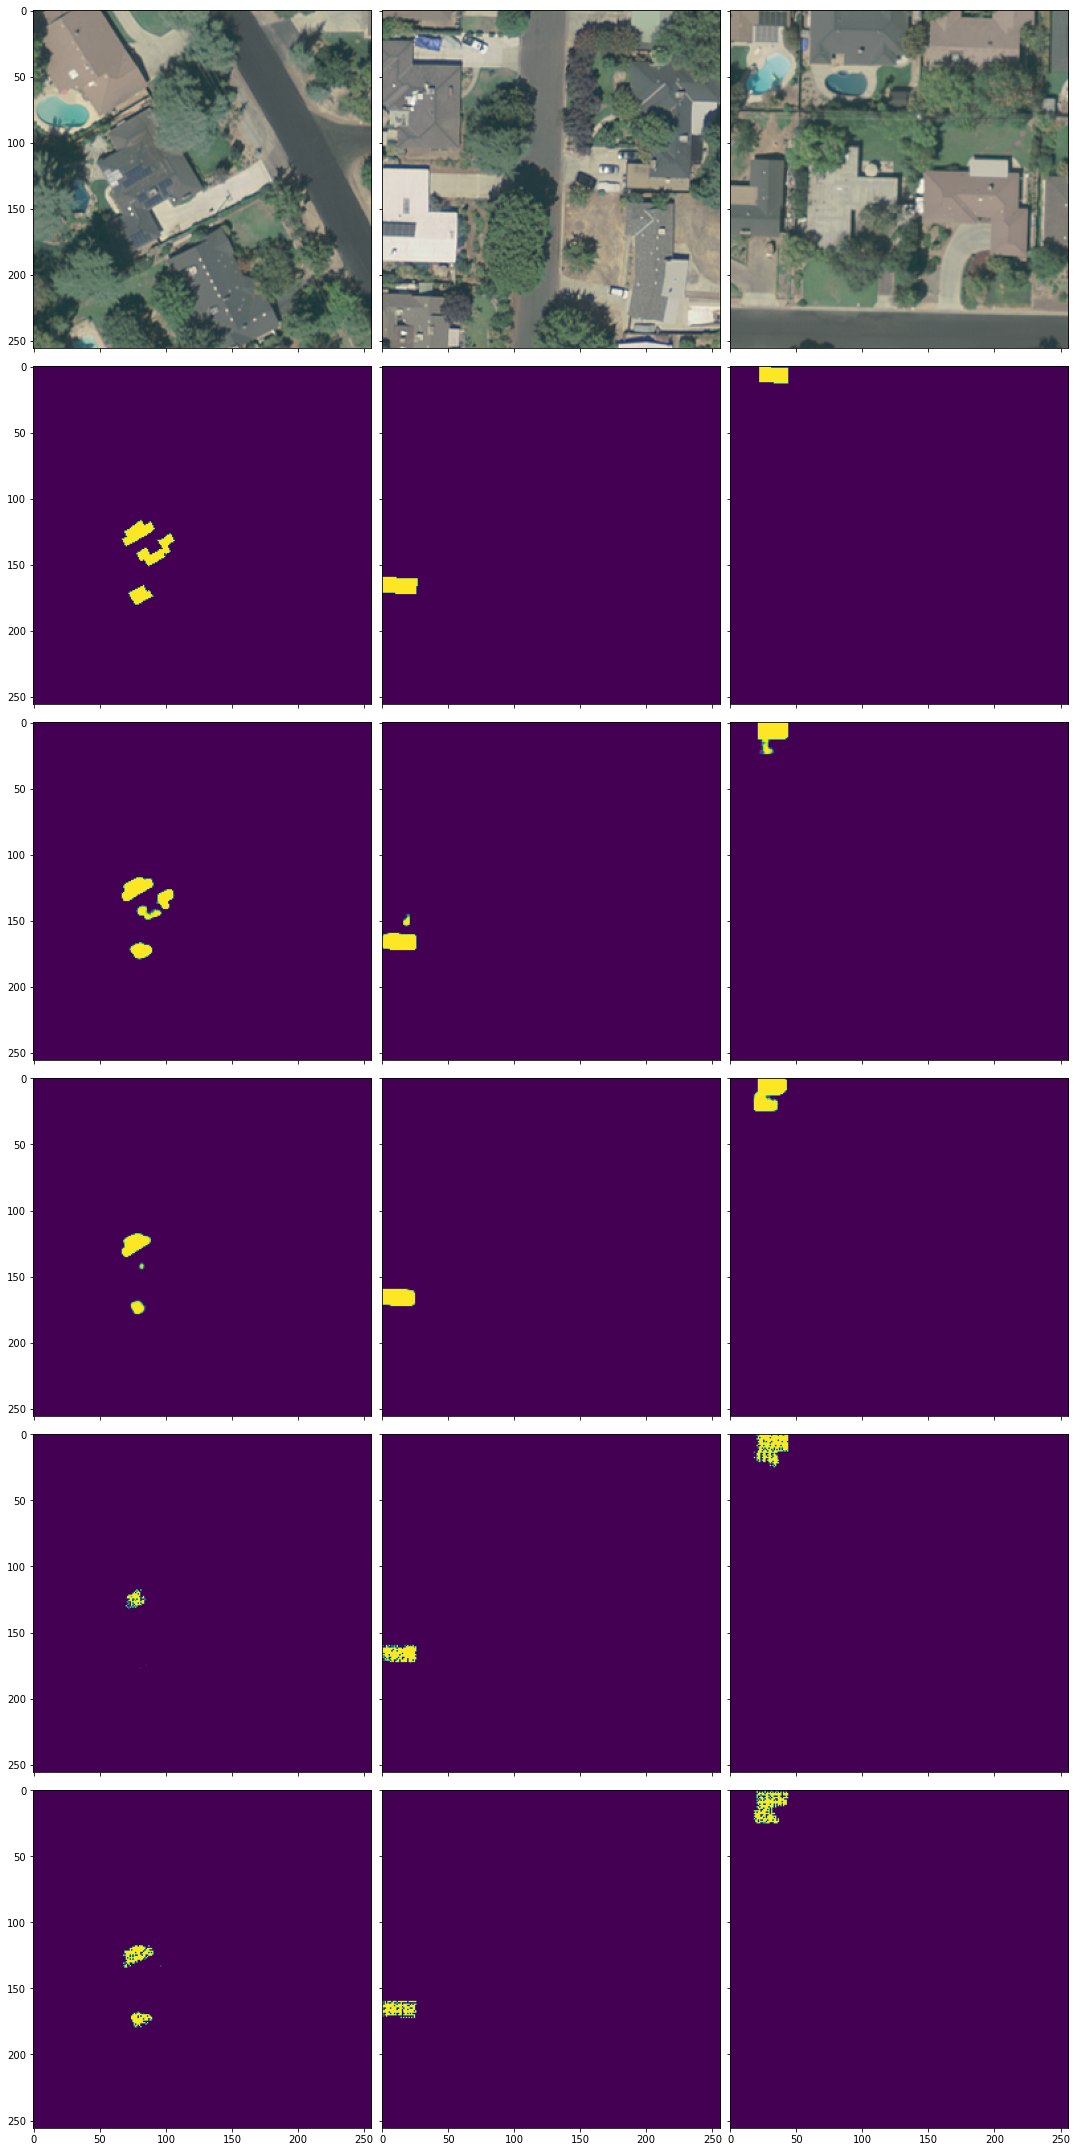
\includegraphics[width=\columnwidth]{resources/png/better.png}
    \caption{Sample of average predictions.}
    \label{fig:average_sample_2}
\end{figure}

\newpage

Images of FIG. \ref{fig:average_sample_2}, are pretty average as well. However, one can note that all four networks seem to detect an array that is not annotated in the third image. By looking closely, we see that it is indeed the case. This raises the question of the quality of our training set.

\newpage

\begin{figure}[h]
    \centering
    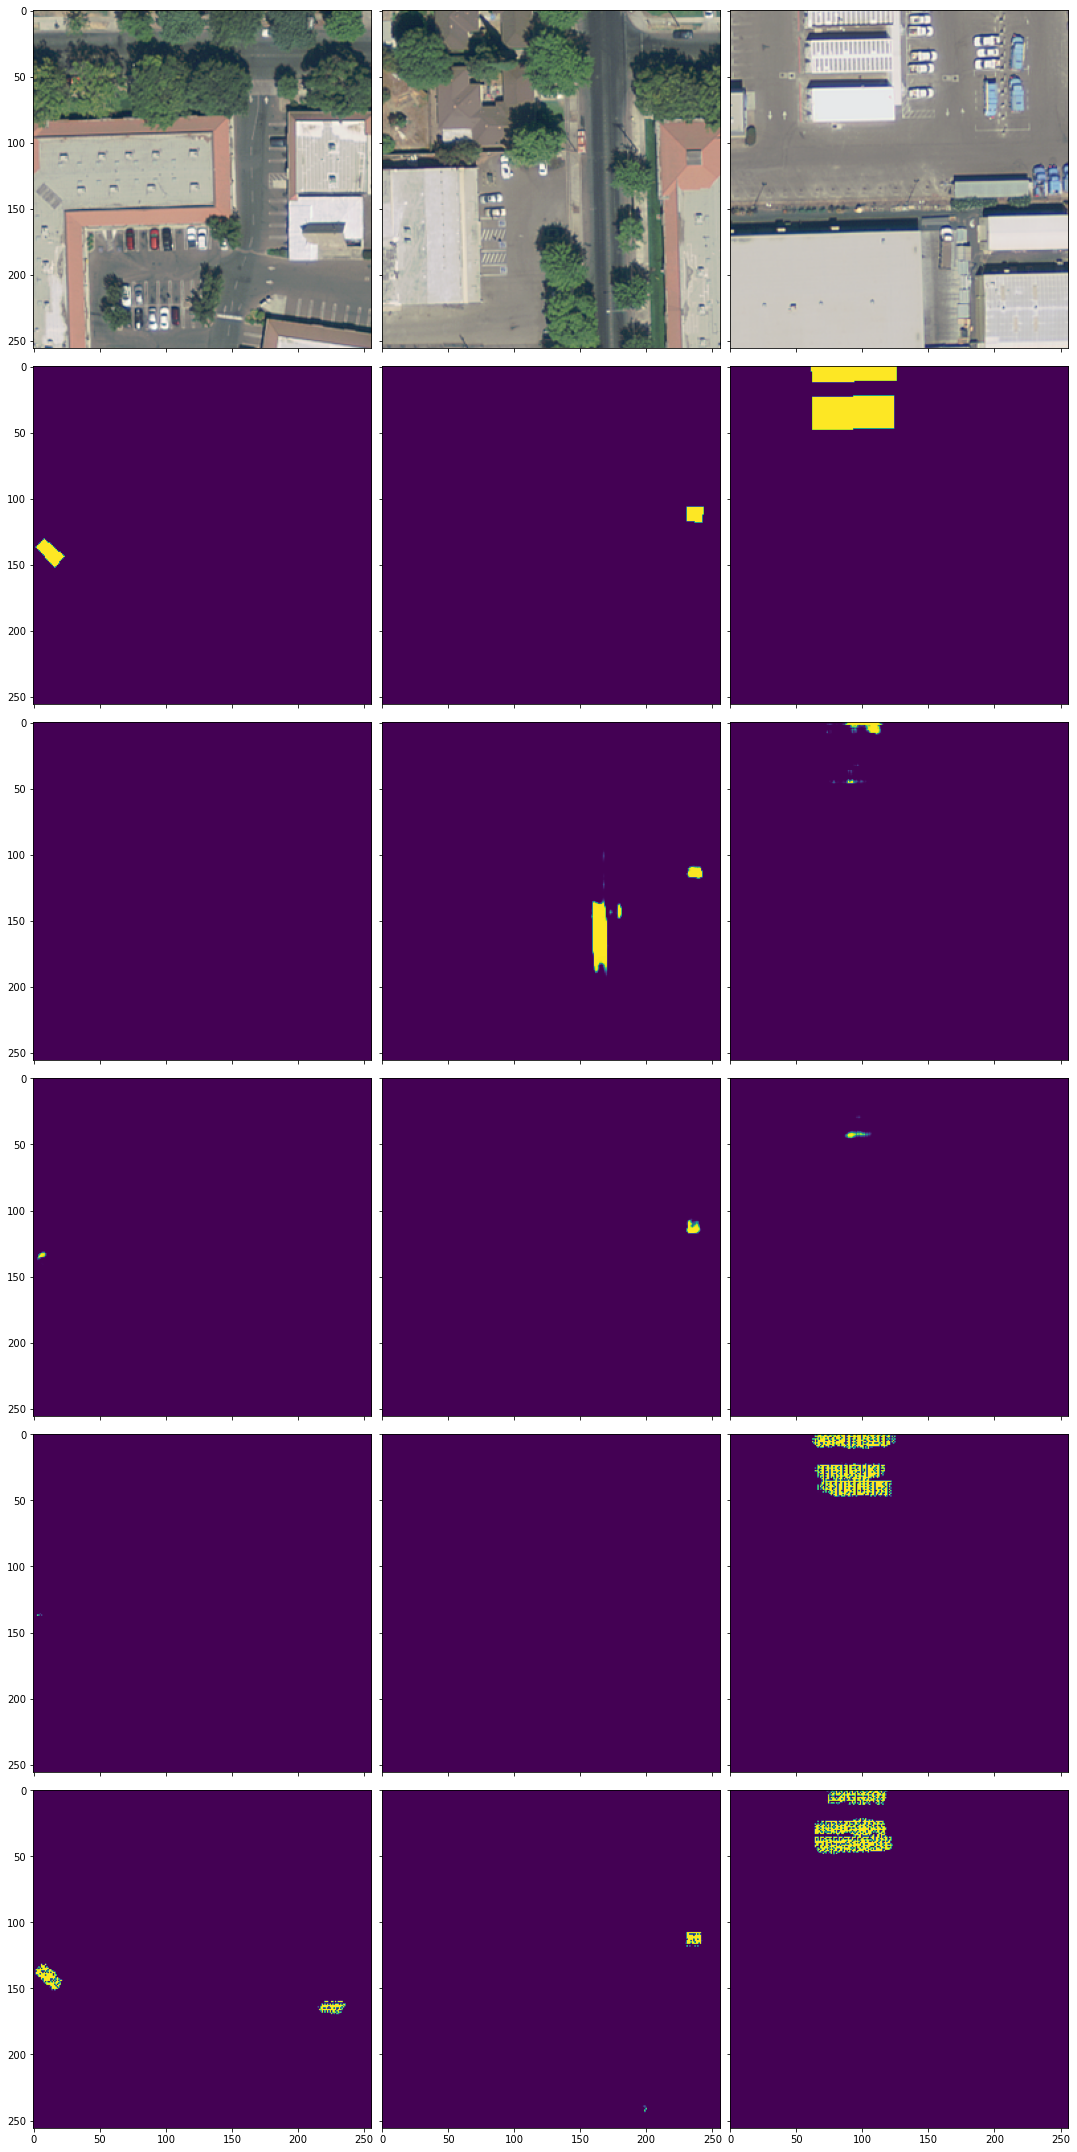
\includegraphics[width=\columnwidth]{resources/png/terrible.png}
    \caption{Sample of bad predictions.}
    \label{fig:bad_sample}
\end{figure}

In FIG. \ref{fig:bad_sample}, the U-Net and Multi-Task U-Net seem to struggle with the third image while SegNet and Multi-Task SegNet don't. This might be due to the unusual look of the annotated arrays.

\end{document}
